\documentclass[conference]{IEEEtran}
\IEEEoverridecommandlockouts
% The preceding line is only needed to identify funding in the first footnote. If that is unneeded, please comment it out.
\usepackage{cite}
\usepackage{amsmath,amssymb,amsfonts}
\usepackage{algorithmic}
\usepackage{graphicx}
\usepackage{textcomp}
\usepackage{xcolor}
\usepackage{url}
\usepackage{multirow}
\usepackage{amsfonts}
\usepackage{threeparttable}
\usepackage{bigstrut}
\usepackage[caption=false,font=normalsize,labelfont=sf,textfont=sf]{subfig}
\usepackage{cleveref}
\def\BibTeX{{\rm B\kern-.05em{\sc i\kern-.025em b}\kern-.08em
  T\kern-.1667em\lower.7ex\hbox{E}\kern-.125emX}}
\begin{document}

\title{INCA: INterruptible CNN Accelerator for Multi-tasking in Robots \\
% {\footnotesize \textsuperscript{*}Note: Sub-titles are not captured in Xplore and
% should not be used}
% \thanks{Identify applicable funding agency here. If none, delete this.}
}

\author{
  % \IEEEauthorblockN{1\textsuperscript{st} Anonymous for Review}
% \IEEEauthorblockA{\textit{dept. name of organization (of Aff.)} \\
% \textit{name of organization (of Aff.)}\\
% City, Country \\
% email address or ORCID}
% \and
% \IEEEauthorblockN{2\textsuperscript{nd} Given Name Surname}
% \IEEEauthorblockA{\textit{dept. name of organization (of Aff.)} \\
% \textit{name of organization (of Aff.)}\\
% City, Country \\
% email address or ORCID}
% \and
% \IEEEauthorblockN{3\textsuperscript{rd} Given Name Surname}
% \IEEEauthorblockA{\textit{dept. name of organization (of Aff.)} \\
% \textit{name of organization (of Aff.)}\\
% City, Country \\
% email address or ORCID}
% \and
% \IEEEauthorblockN{4\textsuperscript{th} Given Name Surname}
% \IEEEauthorblockA{\textit{dept. name of organization (of Aff.)} \\
% \textit{name of organization (of Aff.)}\\
% City, Country \\
% email address or ORCID}
% \and
% \IEEEauthorblockN{5\textsuperscript{th} Given Name Surname}
% \IEEEauthorblockA{\textit{dept. name of organization (of Aff.)} \\
% \textit{name of organization (of Aff.)}\\
% City, Country \\
% email address or ORCID}
% \and
% \IEEEauthorblockN{6\textsuperscript{th} Given Name Surname}
% \IEEEauthorblockA{\textit{dept. name of organization (of Aff.)} \\
% \textit{name of organization (of Aff.)}\\
% City, Country \\
% email address or ORCID}
}

\maketitle

\begin{abstract}
In recent years, Convolutional Neural Network (CNN) has been widely used in robotics, which has dramatically improved the perception and decision-making ability of robots.
In order to implement energy-efficient CNN on embedded systems, a series of CNN accelerators have been designed. However, despite the high energy efficiency on CNN accelerators, it is difficult for robotics developers to use it. Since the various functions on the robot are usually implemented independently by different developers, simultaneous access to the CNN accelerator by these multiple independent processes will result in hardware resource conflicts.

To handle the above problem, we propose an INterruptible CNN Accelerator (INCA) to enable multi-tasking on CNN accelerators. In INCA, we propose a Virtual-Instruction-based interrupt method (VI method) to support multi-task on CNN accelerators. Based on INCA, we deploy the Distributed Simultaneously Localization and Mapping (DSLAM) on an embedded FPGA platform. We use CNN to implement two key components in DSLAM, Feature-point Extraction (FE) and Place Recognition (PR), so that they can both be accelerated on the same CNN accelerator. Experimental results show that INCA enables multi-task scheduling on the CNN accelerator with negligible performance degradation (within 0.3\%). Compared to the layer-by-layer interrupt method, our VI method reduces the interrupt responding latency to 2\%.
\end{abstract}

% \begin{IEEEkeywords}
% component, formatting, style, styling, insert
% \end{IEEEkeywords}

\section{Introduction}
With the development of algorithms and hardware platforms, Convolutional Neural Network (CNN) has greatly improved the perception and decision-making ability of unmanned platform. 
% such as object detection \cite{redmon2018yolov3} and scene segmentation \cite{huang2019mask} in perception, and path planning \cite{chen2017socially} and dynamic obstacle avoidance \cite{kaufmann2018deep} in decision-making.

Distributed Simultaneously Localization and Mapping (DSLAM) is a basic task for many multi-robot applications, and is a hot topic in robotics. There are two key modules which consume most of the computation: Feature-point Extraction (FE) and Place Recognition (PR). 
FE provides the feature-points for the Visual Odometry (VO) to calculate the relative pose between two adjacent frames. PR generates the compact image representation, which produces the candidate place recognition matches between different robots. 
Recent works use CNN to extract feature-points  ~\cite{detone2018superpoint, simo2015discriminative, yi2016lift} and generate the place representation code  ~\cite{arandjelovic2016netvlad, radenovic2018fine}. 
The CNN-based feature-point extraction method, SuperPoint  ~\cite{detone2018superpoint}, achieves 10\%-30\% higher matching accuracy compared with the popular handcrafted extraction method, ORB ~\cite{Mur-Artal:2017281}.
The accuracy of the place recognition code from another CNN-based method, GeM  ~\cite{radenovic2018fine}, is also about 20\% better than the handcrafted method, rootSIFT  ~\cite{jegou2014triang}.

However, CNN is computation consuming. A single inference forward of the CNN-based SuperPoint feature-point extraction consumes 39G operations  ~\cite{detone2018superpoint}, and a single inference forward of the CNN-based GeM  place recognition consumes 192G operations  ~\cite{radenovic2018fine}.
Thus, specific hardware architectures on FPGA  ~\cite{guo2017angel,yu2018instruction,li_high_2016,qiu2016going,lu_evaluating_2017} are designed to deploy CNN on the embedded system.
With the help of network quantization and on-chip data reuse, the speed of CNN accelerators on embedded FPGA achieves 3TOP/s  ~\cite{lu_evaluating_2017}, which can support the real-time execution of CNN-based feature-point extraction  ~\cite{detone2018superpoint}.
However, these CNN accelerators are designed and optimized to accelerate a single CNN. They can not automatically schedule two or more tasks simultaneously. 


\begin{figure}[t]
	\centering
    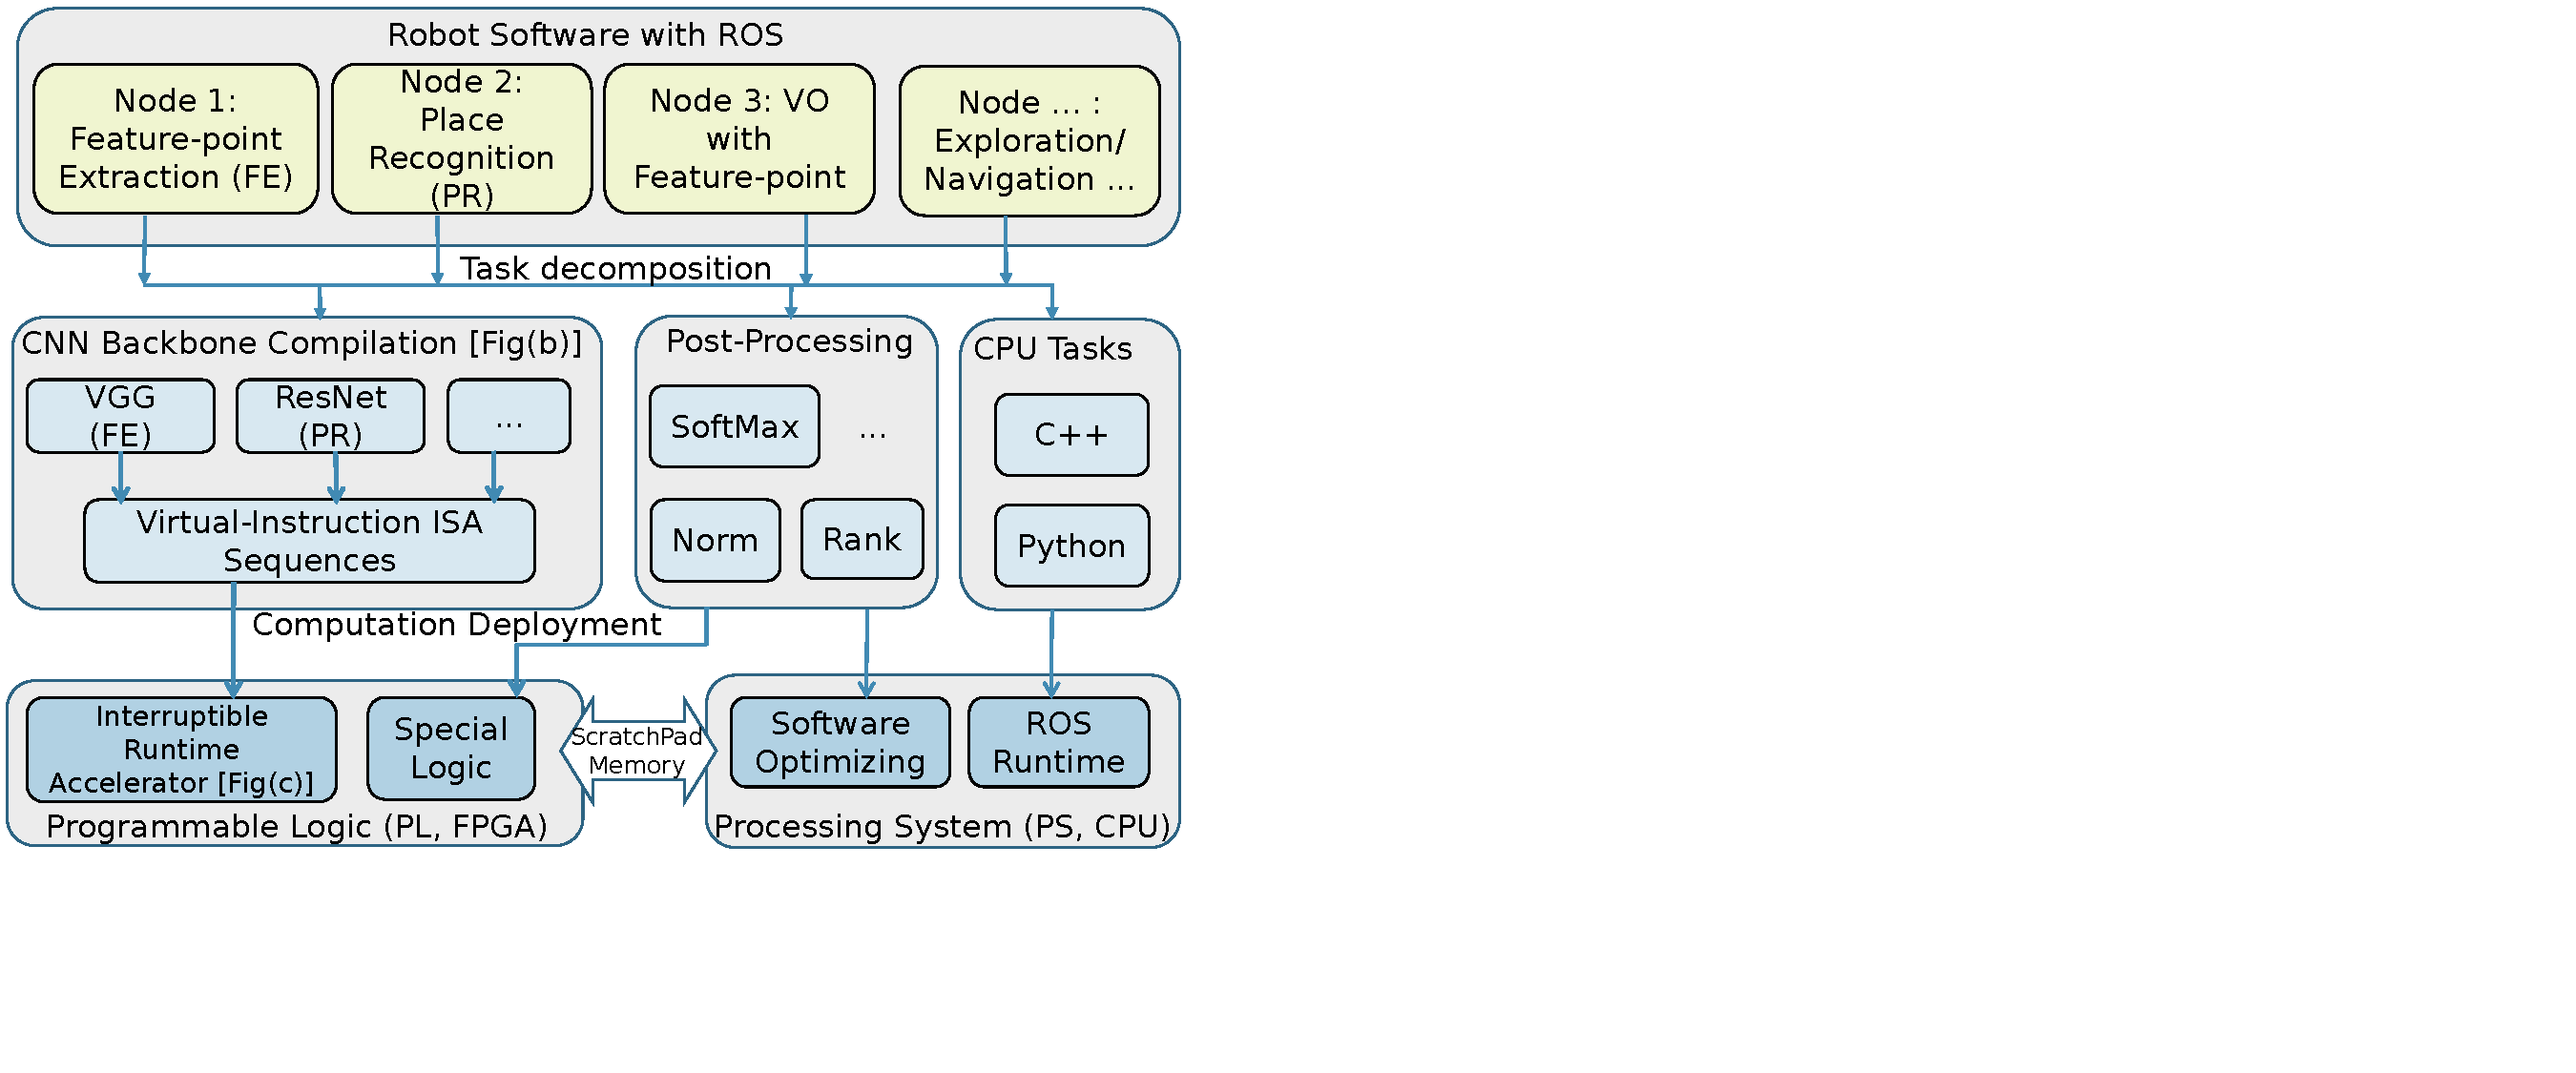
\includegraphics[width=0.99\linewidth]{fig/inca.pdf}
    \caption{ INCA framework. At task decomposition step, the operations in different ROS nodes are separated to CNN backbones, CNN Post-Processing, and Other CPU Tasks. At computation deployment, the CNN backbone and Post-Processing are deployed with hardware modules and software optimizing.  
    }
	\label{fig:inca}
\end{figure}

In order to facilitate robotic researchers to run different CNN tasks simultaneously on the FPGA accelerator, the accelerator should support the following features:

\textbf{Multi-thread:} Because different components in a robot are from different developers, thus, Robot Operating System (ROS)  ~\cite{quigley2009ros} is proposed as a middleware to fuse these independent components, and is widely used by robotic researchers. Each component is considered as an independent thread in ROS. Different threads should have independent access to the accelerator without knowing the status of others.

\textbf{Finishing before deadline:} In a robot, some tasks must be completed within the specified hard deadlines, such as feature-point extraction. The moving robot's perception, including estimation of itself's location and the obstacles' position, is based on the feature-points. If the feature point extraction is not completed before the deadline, the robot can not estimate the surrounding environment, causing collisions or even damage. Those critical tasks with a more stringent headline need to be performed prior to some non-critical tasks ~\cite{RamsauerKLM17}. In DSLAM, the priority of feature-point extraction (FE) is higher than that of place recognition (PR). Because PR is only related to efficiency, yet FE ensures system safety.

To address above challenges, we propose an INterruptible CNN Accelerator (INCA) for rapid deployment of robot application on FPGA. 
The work flow of INCA is illustrated in \Cref{fig:inca}. 
INCA is a two-step framework for mapping software to embedded FPGA. 
The first step is the task decomposition, which decomposes the computation in ROS nodes into different computation types, including CNN backbones, CNN post-processing, and other CPU tasks.
The second step is to deploy the computation onto the FPGA. 
The CNN backbones of different tasks, such as the VGG model  ~\cite{kim2016accurate} in SupoerPoint feature-point extraction  ~\cite{detone2018superpoint} and the ResNet101 model  ~\cite{he2016deep} in GeM place recognition  ~\cite{radenovic2018fine}, are compiled to the interruptible Virtual-Instruction Instruction Set Architecture (VI-ISA), which runs on the CNN accelerator. The VI-ISA is a simple extension of the original ISA, in which the extension method is not limited to a specific original ISA. Thus, the virtual-instruction-based interrupt can be easily applied to various instruction-based CNN accelerators  ~\cite{yu2018instruction,qiu2016going}, such as Angel-Eye ~\cite{guo2017angel} and DPU ~\cite{dpu}.


% The CNN backbones of different tasks, such as the VGG model  ~\cite{kim2016accurate} in SupoerPoint ~\cite{detone2018superpoint} and the ResNet101 model  ~\cite{he2016deep} in GeM  ~\cite{radenovic2018fine}, are compiled to the interruptible Virtual-Instruction Instruction Set Architecture (VI-ISA), which runs on the CNN accelerator.
% The VI-ISA is a simple extension of the original ISA, in which the extension method is not limited to a specific original ISA. Thus, the virtual-instruction-based interrupt can be easily applied to various instruction-based CNN accelerators  ~\cite{yu2018instruction,qiu2016going}, such as Angel-Eye ~\cite{guo2017angel} and DPU ~\cite{dpu}.


In conclusion, INCA facilitate robotic researchers to run different CNN tasks simultaneously on the FPGA with the following contributions:
\begin{itemize}
\item We propose a \textbf{virtual-instruction-based} interrupt method to make the CNN accelerator support dynamic multi-task scheduling by priority. The method solves the hardware resources conflicts when accelerating different CNN tasks on ROS~\cite{quigley2009ros}.
% \item We only needs to modify the instruction fetch module of the CNN accelerator in hardware to support interrupt. Thus, it is easy to be extended to different instruction-driven CNN accelerators.
\item We propose a CNN-based DSLAM system to evaluate INCA. CNN-based methods for feature-point extraction (FE) and place recognition (PR) are accelerated with FPGA on ROS platform. With the help of the unified interface in ROS, these CNN-based methods can be easily used by other developers in different applications.
\end{itemize}
% In terms of perception, CNN has surpassed traditional algorithms in tasks such as object detection \cite{redmon2018yolov3} and scene segmentation \cite{huang2019mask}. 
% In decision-making, CNN also performs well in path planning \cite{chen2017socially} and dynamic obstacle avoidance \cite{kaufmann2018deep}.



\section{Related Work}
% In order to deploy the robot task on embedded systems, a series of works have involved special hardware architectures for high energy efficiency. 
% There are two kinds of hardware design for embedded moving robot: one is to design a special acceleration for a specific task; the other is to design CNN accelerators and use CNN to do the task.

% \subsection{ Accelerators for a specific robot task }

% The feature-point extraction (FE) operation is the fundamental component of a vision-based robot, and is also one of the most time-consuming components \cite{fang2017fpga}.
% Some previous works design hardware architectures for FE.
% SRI-SURF \cite{jia2016sri} optimizes the memory access to speed up SURF \cite{bay2006surf} feature-point extraction. 
% \cite{fang2017fpga} directly implements ORB on FPGA using HLS. eSLAM \cite{liu2019eslam} optimizes the ORB algorithm and designs hardware for better performance.
% Some other works design architectures for the entire robot system. Hero \cite{shi2018hero} is a framework for navigation and laser-based robot and cannot support vision-based robots that are much more lightweight and cheaper. 
% \cite{li2019879gops} introduces CNN accelerators for the vision-based robot. 
% However, the CNN accelerator in this work \cite{li2019879gops} is only used for feature-point extraction, and the accelerator is not to support different tasks at the same time. 
% Deploying multiple CNNs on the robotic accelerator can expand the functions of robots, without designing hardware for specific functions.



% \subsection{ CNN accelerators }

To accelerate CNN, some previous works design frameworks to generate a specific hardware architecture for a target CNN, based on RTL \cite{li_high_2016} or HLS \cite{lu_evaluating_2017}. These works need to reconfigure the FPGA to switch between different CNN models. The reconfiguration consumes seconds \cite{FPGAPerformance}, which is unacceptable for the real-time system.
Some other works design instruction-driven accelerators \cite{yu2018instruction,qiu2016going,guo2017angel,dpu}, making rapid switching possible by providing different instruction sequences. 
However, the CNN tasks on previous instruction-driven CNN accelerators are not interruptible, resulting in the latency-sensitive high-priority task waiting for the low-priority task to finish. 
This inability of CNN accelerators to support multi-task makes it difficult for robotic researchers to use embedded FPGA.

\section{INCA Frame work}

% \begin{figure}[t]
% 	\centering
% % \vspace{-0.1cm} 
% % \setlength{\abovecaptionskip}{0cm} 
% % \setlength{\belowcaptionskip}{-0.2cm} 
% 	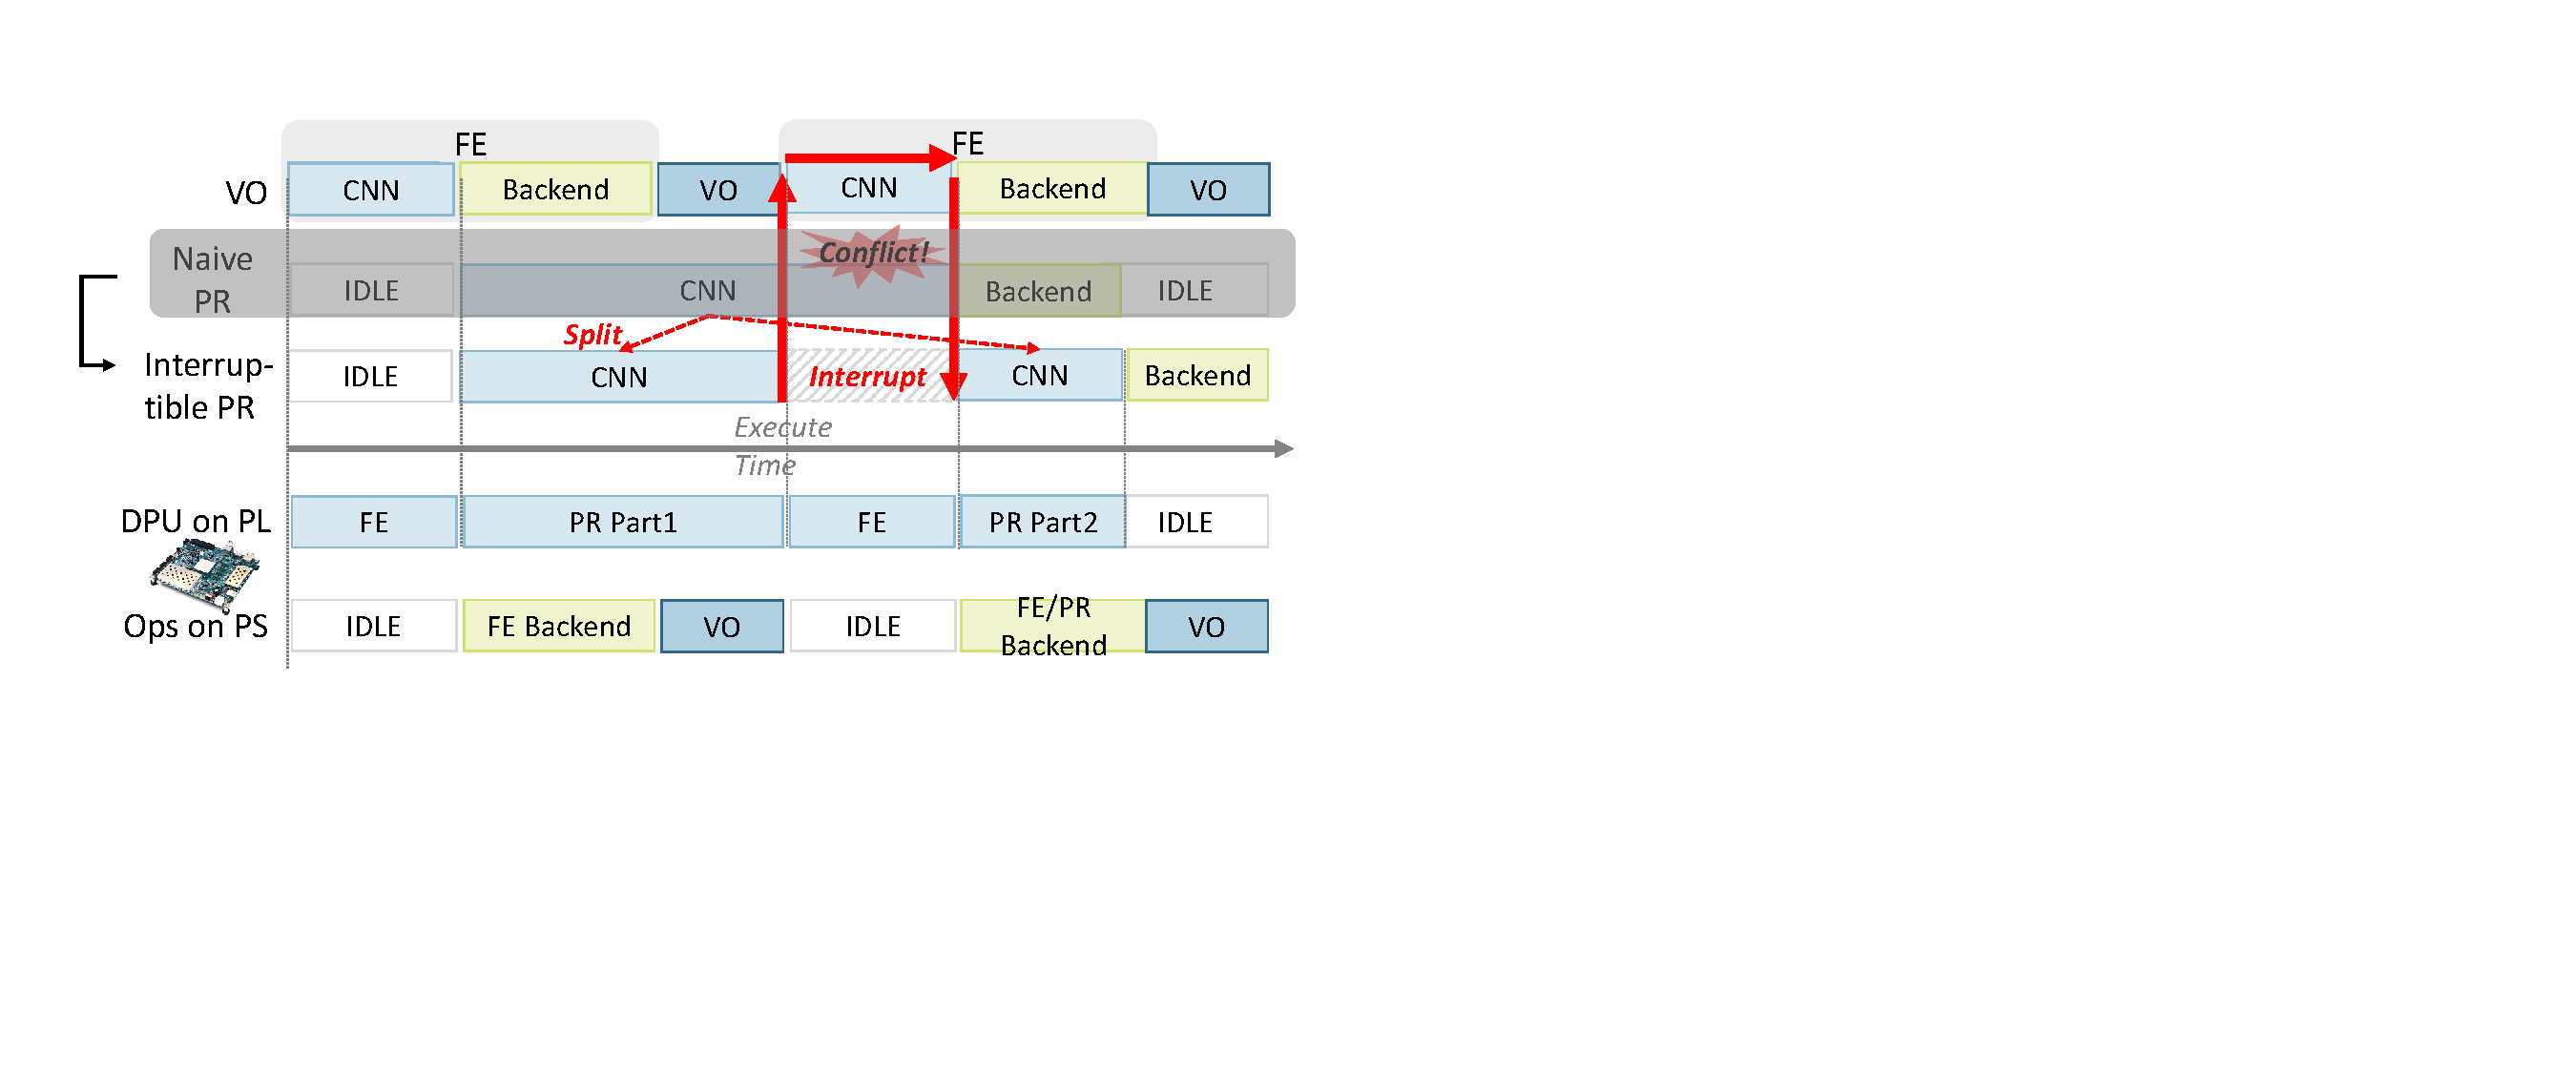
\includegraphics[width=0.95\linewidth]{fig/interDPR.pdf}
% \caption{Interruption to solve the hardware resources conflicts. 
% % When a high-priority task (FE) is started before the low-priority task (PR) is completed, the CNN accelerator backs up the status of PR to memory, and processes the FE task. When the high-priority task is completed, the low-priority task resumes and continues.
% }
% 	\label{fig:interDPR}
% \end{figure}

% \begin{figure}[t]
% 	\centering
% 	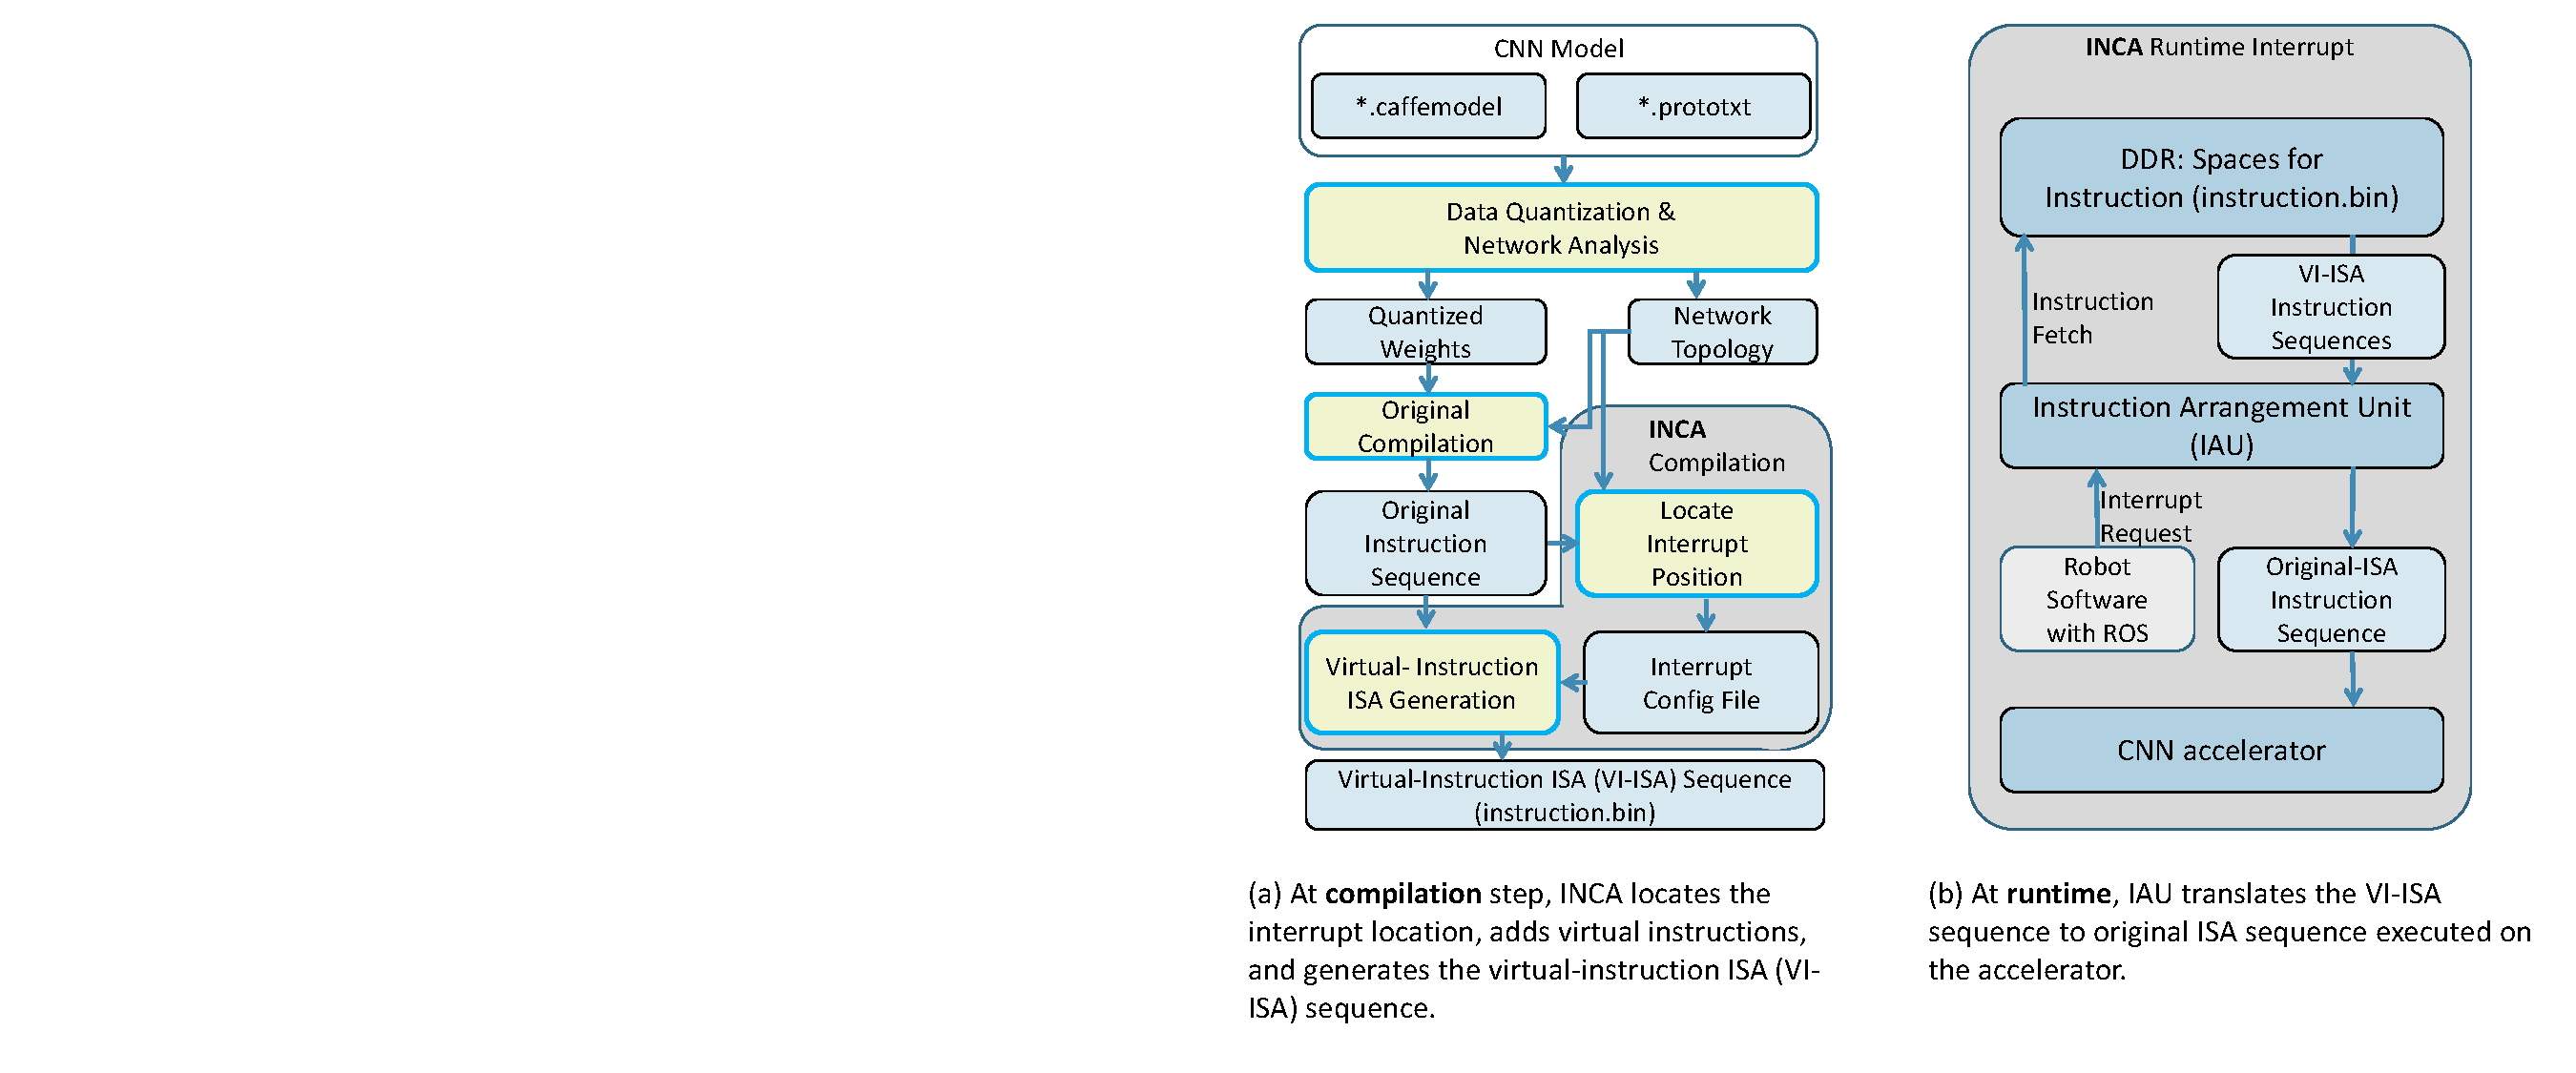
\includegraphics[width=0.95\linewidth]{fig/inca_acc.pdf}
% \caption{INCA framework with Virtual-Instruction (VI). 
% }
% 	\label{fig:inca_acc}
% \end{figure}


 Although ROS is becoming the fundamental software platform for robotics, the independence between different ROS nodes brings \textbf{hardware resources conflicts} to access the hardware accelerator. \Cref{fig:inca}(a) shows the time diagram of scheduling feature-point based visual odometry (VO) and Place Recognition in DSLAM system. The feature-point extraction (FE) and Place Recognition (PR) are impelmented in CNN and deployed to the CNN accelerator. In the native accelerator (the shadow part in \Cref{fig:inca}(a)), the threads of FE and PR may need to process CNN at thesame time, and the simultaneous requests of the acceleratorwill lead to hardware resources conflicts. 

\Cref{fig:inca}(a) also illustrates the idea of interrupt to schedule two CNN tasks. In the process of running a low-priority network (PR), the software may send an execution request for the high-priority task (FE). The interrupt enables the CNN accelerator to backup the running state of the low-priority PR network. Then the accelerator switches to the high-priority FE network. After the high-priority task (FE) completes, the low-priority task (PR) is restored to the accelerator and continues to execute.


\Cref{fig:inca}(c) details the INCA compilation step and runtime interrupt. Caffe \cite{jia2014caffe} is a popular software framework for CNN, and the *.caffemodel/*.prototxt files define the network parameters and structure in Caffe. The previous deployment process, such as Angel-Eye \cite{guo2017angel} and DPU \cite{dpu}, quantizes the weights, and analyze the network topology. The original compiler translates the network topology and the quantization information into the original ISA sequence. INCA goes further than previous CNN compilers. It selects the optimized interrupt positions in the original instruction sequence, and adds virtual instructions at these positions to enable accelerator interrupt. After that, the original instruction sequence and the added virtual instructions are wrapped to the new interruptible VI-ISA. The wrapped VI-ISA instructions are dumped into a file (instruction.bin), and can be loaded into the instruction spaces on FPGA's DDR.


As illustrated in \Cref{fig:inca}(d), at runtime, an Instruction Arrangement Unit (IAU) in hardware listens to the interrupt request from ROS software, fetches the corresponding VI-ISA interruptible instructions and translates them to the original ISA executed on the CNN accelerator. 
Although INCA can be applied to various instruction-based CNN accelerators, we implement and evaluate it based on Angel-Eye \cite{guo2017angel}.
% The detail of the Virtual-Instruction ISA (VI-ISA) and instruction arrangement unit (IAU) is introduced in \Cref{sec:cnninterrupt}. Although INCA can be applied to various instruction-based CNN accelerators, we implement and evaluate it based on Angel-Eye \cite{guo2017angel}.




\section{Virtual-instruction-based Accelerator Interrupt}
\label{sec:cnninterrupt}


% Table generated by Excel2LaTeX from sheet 'Sheet3'
\begin{table}[t]
	\centering
	\scriptsize
	\caption{Description for the basic instructions}
% Table generated by Excel2LaTeX from sheet 'Sheet5'
% Table generated by Excel2LaTeX from sheet 'Sheet5'
\begin{tabular}{|p{4em}|p{12em}||p{6em}|p{6em}|}
	\hline
	Type  & Description & Backups & Recovery \bigstrut\\
	\hline
	LOAD\_W  & Load weights/bias from DDR to on chip weight buffer. & -     & Weight / Inputdata \bigstrut\\
	\hline
	LOAD\_D  & Load input featuremaps from DDR to on chip weight buffer. & -     & Weight / Inputdata \bigstrut\\
	\hline
	CALC\_I & Calculate intermediate results for some output channels from partial  input channels. & Previous final results / Intemediate data  & Weight / Inputdata /  intemediate data \bigstrut\\
	\hline
	CALC\_F & Calculate the results for some output channels from all input channels. & Finial results & Weight / Inputdata \bigstrut\\
	\hline
	SAVE  & Save the results from on-chip data buffer to DDR. & -     & Weight / Inputdata \bigstrut\\
	\hline
	\end{tabular}%
	
	\label{tab:instr}%
  \end{table}%
  

% \begin{figure}[t]
% 	\centering
% 	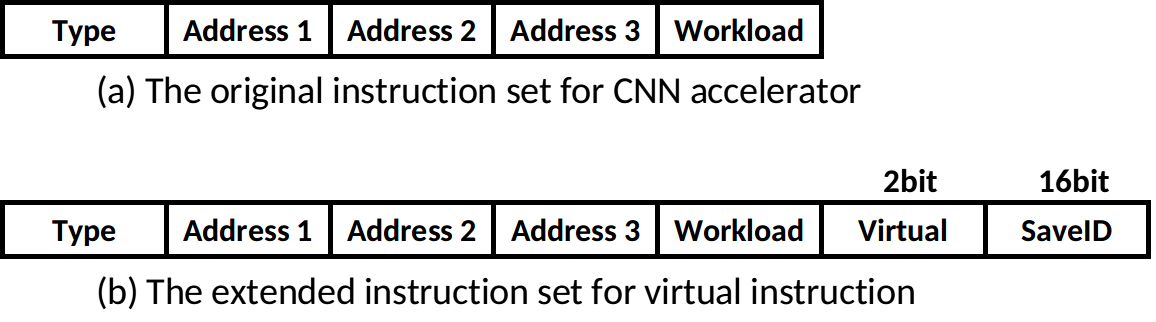
\includegraphics[width=0.9\linewidth]{fig/instructions.png}
% 	\caption{Original and Virtual-Instruction ISA.}
% 	\label{fig:instructions}
% \end{figure}



\subsection{ Instruction Driven Accelerator }
\label{sec:instrAcc}
There are three categories of instruction in the instruction-driven accelerator: LOAD (LOAD\_W / LOAD\_D), CALC (CALC\_I / CALC\_F), and SAVE  ~\cite{guo2017angel,qiu2016going,yu2018instruction}. The instruction description of each kind of instruction is listed in \Cref{tab:instr}. 

Each CALC  instruction,  including CALC\_I and CALC\_F, processes the convolution according to the hardware parallelism with $Para_{height}$ lines from $ Para_{in} $ input channels to $ Para_{out}$ output channels. $Para_{height}$, $ Para_{in} $, and $ Para_{out} $ are the parallelism along the height, input channel and output channel dimensions, which is determined by the hardware and original ISA. The convolution of the last $ Para_{in} $ input channels is CALC\_F, and the convolutions for the former input channels are CALC\_I, as illustrated in \Cref{fig:singlesave}(a). The CALC\_F and the CALC\_I instructions for the same output channels, as well as the LOAD instructions for corresponding input feature-maps and weights, are considered as a \textbf{CalcBlob}.


\begin{figure}[t]
    \centering
	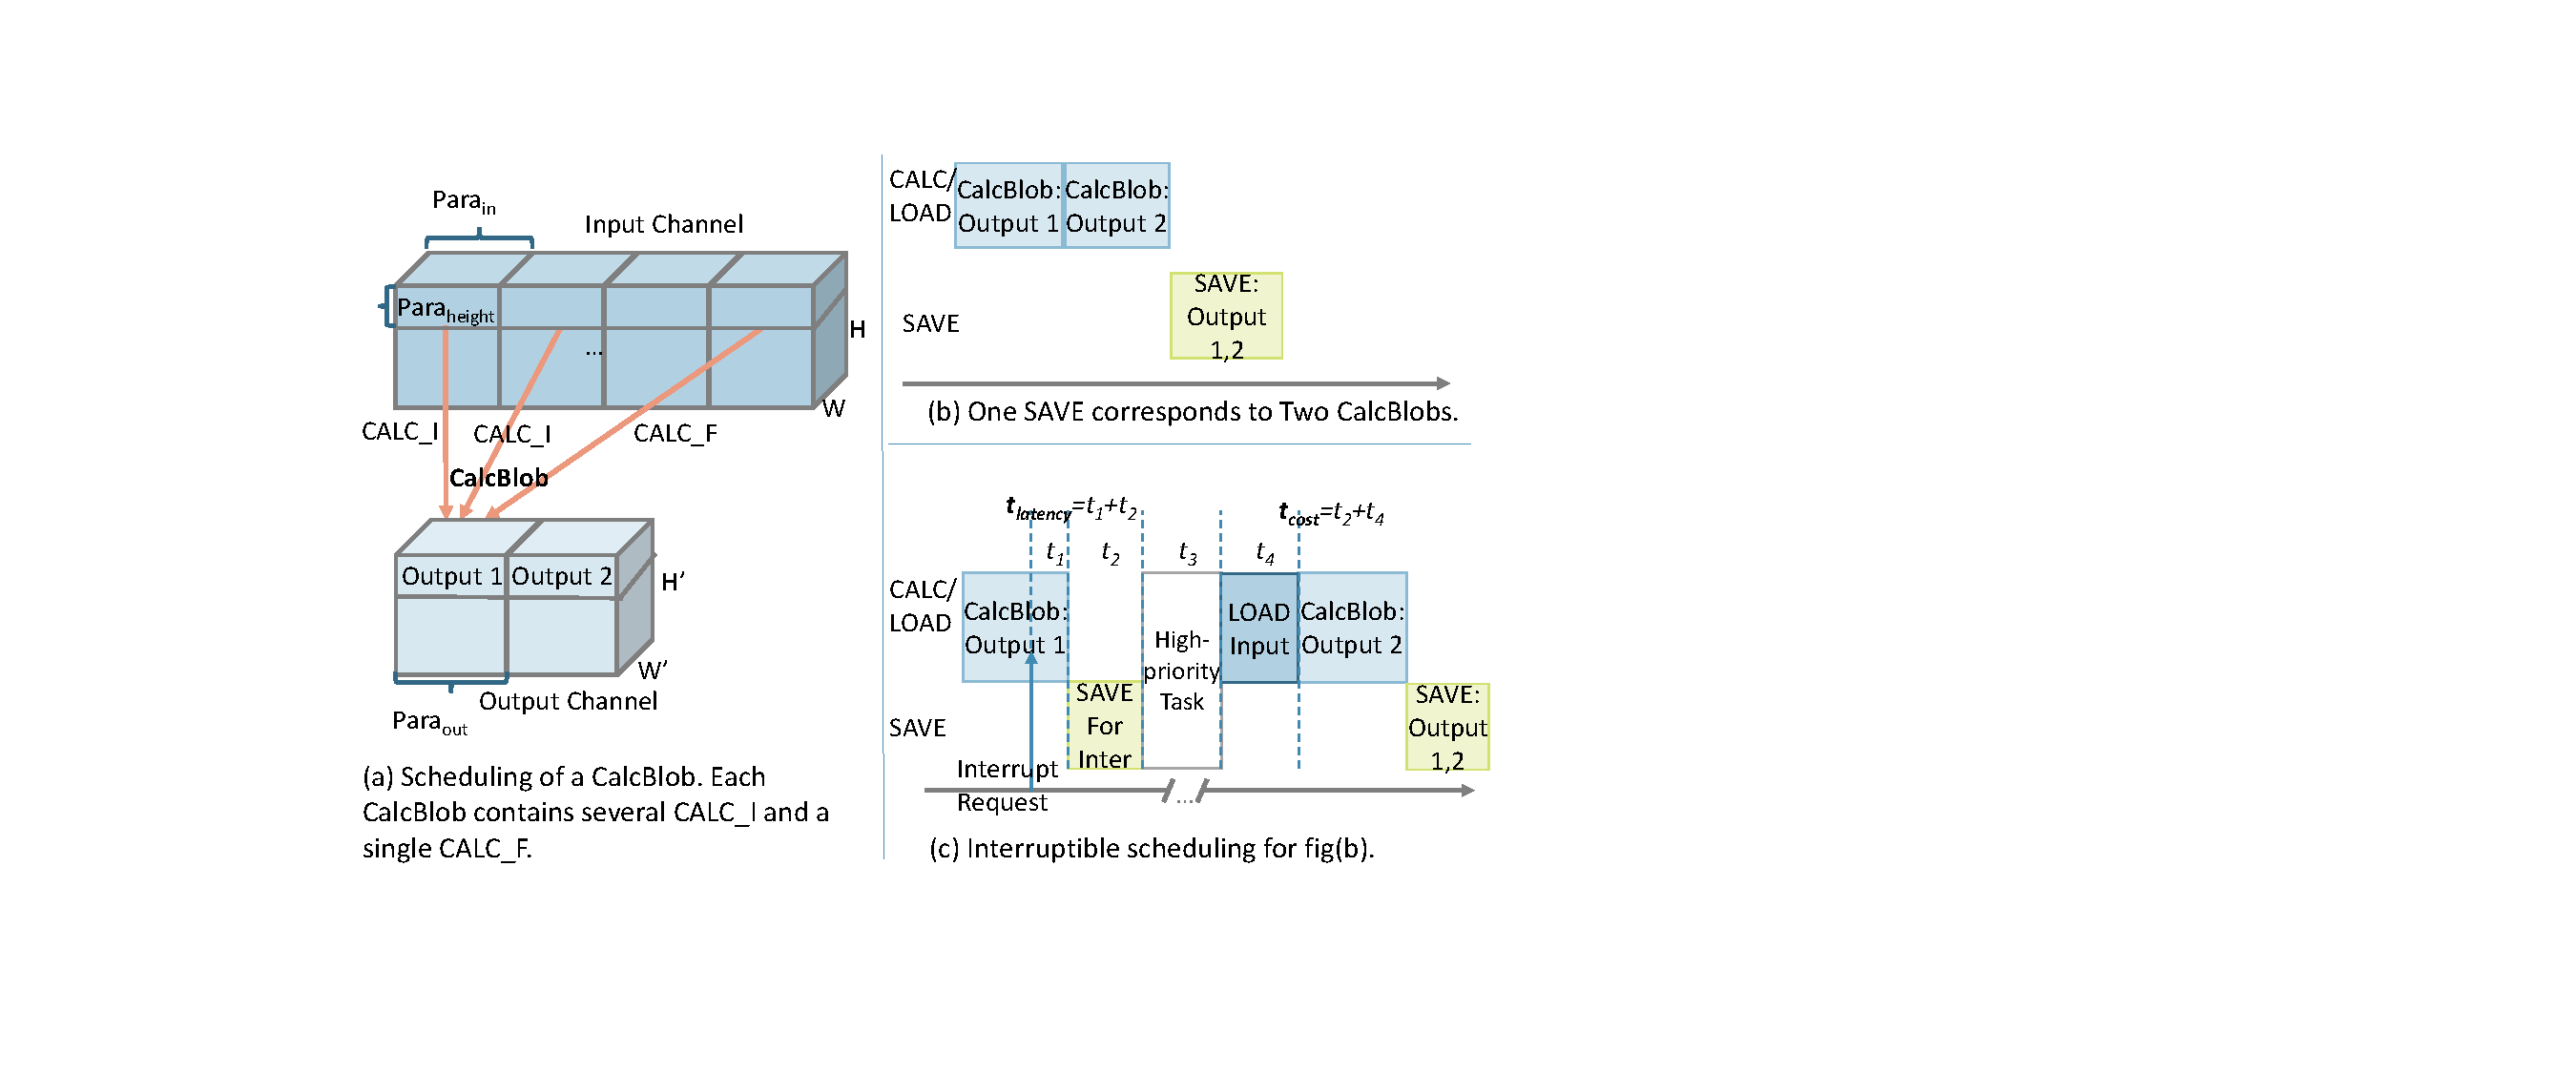
\includegraphics[width=1.04\linewidth]{fig/singlesave.pdf} 	
    \caption{
		Scheduling Illustration
    }
	\label{fig:singlesave}
\end{figure}

\subsection{How To Interrupt: Virtual Instruction}
\label{sec:howinter}

There are four stages to handle interrupt. For the instruction flow illustrated in \Cref{fig:singlesave}(b), the interrupt stages are shown in \Cref{fig:singlesave}(c), including: (1) Time for finishing the current operation, $t1$. (2) Time to backup, $t2$. (3) Time for the high-priority task, $t3$. (4) Time to restore the low-priority task ,$t4$. The the latency to respond the interrupt is $t_{latency} = t_1+t_2$. The extra cost for interrupt is $t_{cost}=t_2+t_4$. 
There are different methods to implement interrupt in CNN accelerators.

\textbf{CPU-Like.}
When an interrupt request occurs in CPU, CPU backs up all the on-chip registers to DDR. However, there are only tens of registers in CPU, and the volume of the backed-up data is less than 1 KB  ~\cite{furber2000arm}. In CNN accelerators, there are several $MB$ of on-chip caches  ~\cite{qiu2016going, guo2017angel} for input feature-maps and weights. 
% If all on-chip caches are backed-up/recovered, the cost of data transfer in the accelerator is much higher than that of CPU. 
Thus, the extra data transfer increases both the interrupt response latency($t_{latency}$) and the additional cost ($t_{cost}$).

\textbf{Layer-by-layer.}
Most accelerators run the CNN layer by layer  ~\cite{qiu2016going,guo2017angel}. 
There is no extra data transfer for the accelerator to switch between different tasks after each layer, thus, $t_{cost}=0$. 
However, the position of the interrupt request is irregular and unpredictable. When an interrupt occurs inside a CNN layer, the CNN accelerator needs to finish the whole layer before switching, which leads to the high response latency($t_{latency}$).

% The latency to respond the interrupt and the performance degradation of the CPU-like interrupt and Layer-by-layer method will be evaluated in \Cref{sec:experiments}.

We propose the \textbf{virtual-instruction-based} method (VI method) to enable low-latency interrupt. 
% Different from the CPU-like interrupt, which backup/recovery all the on-chip caches, only the on-chip cache which is still needed in future execution will be backed-up and restored. So that the amount of data transfer is much lower than that of CPU-like interrupt.
To reduce the interrupt response latency, our virtual-instruction-based method is interruptible inside each layer. We add some virtual instructions to the original instruction sequence to enable the interrupt.
The virtual instructions, which contain the backup and recovery instructions, are responsible for backing up and restoring on-chip caches. 

% \textbf{Virtual SAVE} instructions back up the intermediate results from partial input channels or the final output results. There is no need to back up the input feature-maps and weights, because these inputs are already stored in DDR. 

% \textbf{Virtual LOAD} instructions restore the input feature-maps from DDR to on-chip caches, because input featuremaps are loaded by one CalcBlob, and shared across subsequent CalcBlobs.
% , and thus the subsequent CalcBlobs do not read the input feature-maps. 
% Virtual LOAD instructions also need to restore the intermediate results from partial input channels backed up by the virtual SAVE instructions.


\subsection{ Where To Interrupt: After SAVE/CALC\_F }
\label{sec:whereinter}
% The virtual-instruction-based method has two potential factors that may lead to system performance degradation: 1) The extra data transfer to backup/restore running status takes up additional bandwidth resources. 2) The instruction fetching for the virtual instructions also uses bandwidth resources.
%  Even they are skipped and discarded.
% To address the above problems of virtual-instruction-based method, 
We analyze the interrupt cost and select the positions of adding the virtual instructions.
The backup/recovery data for different interrupt positions at each kind of instruction are listed in the Backup/Recovery columns of \Cref{tab:instr}.

When an interruption occurs at \textbf{LOAD}, the newly loaded data are immediately flushed when running the high-level CNN, leading to bandwidth waste.

Compared with CALC\_I, when an interrupt occurs at \textbf{CALC\_F}, there are no intermediate results. 
Although it is necessary to back up the unsaved final results which are generated by previous CALC\_F, these results will be stored in DDR through the subsequent original SAVE instruction.
If the accelerator can record the interrupt status, we can modify the address and workload when executing subsequent original not-virtual SAVE instruction.
Thus, we can avoid the repetitive transmission of the final output results.

The overhead of interrupt after \textbf{SAVE} is only to transfer input data from DDR to the on-chip caches. 

In order to minimize the cost of interrupt, we make the CNN interruptible after the SAVE or CALC\_F. This method only introduces extra data transfer to recovery input data without any extra backup data. Thus, $t_{cost} = t_4$, in our virtual-instruction-based interrupt.

% \begin{figure*}[t]
% 	\centering
% 	\subfloat[ $t_1$ for Layer-By-Layer method. ]{ \label{fig:t1all}
% 		\begin{minipage}[t]{0.45\linewidth}
% 			\centering
% 	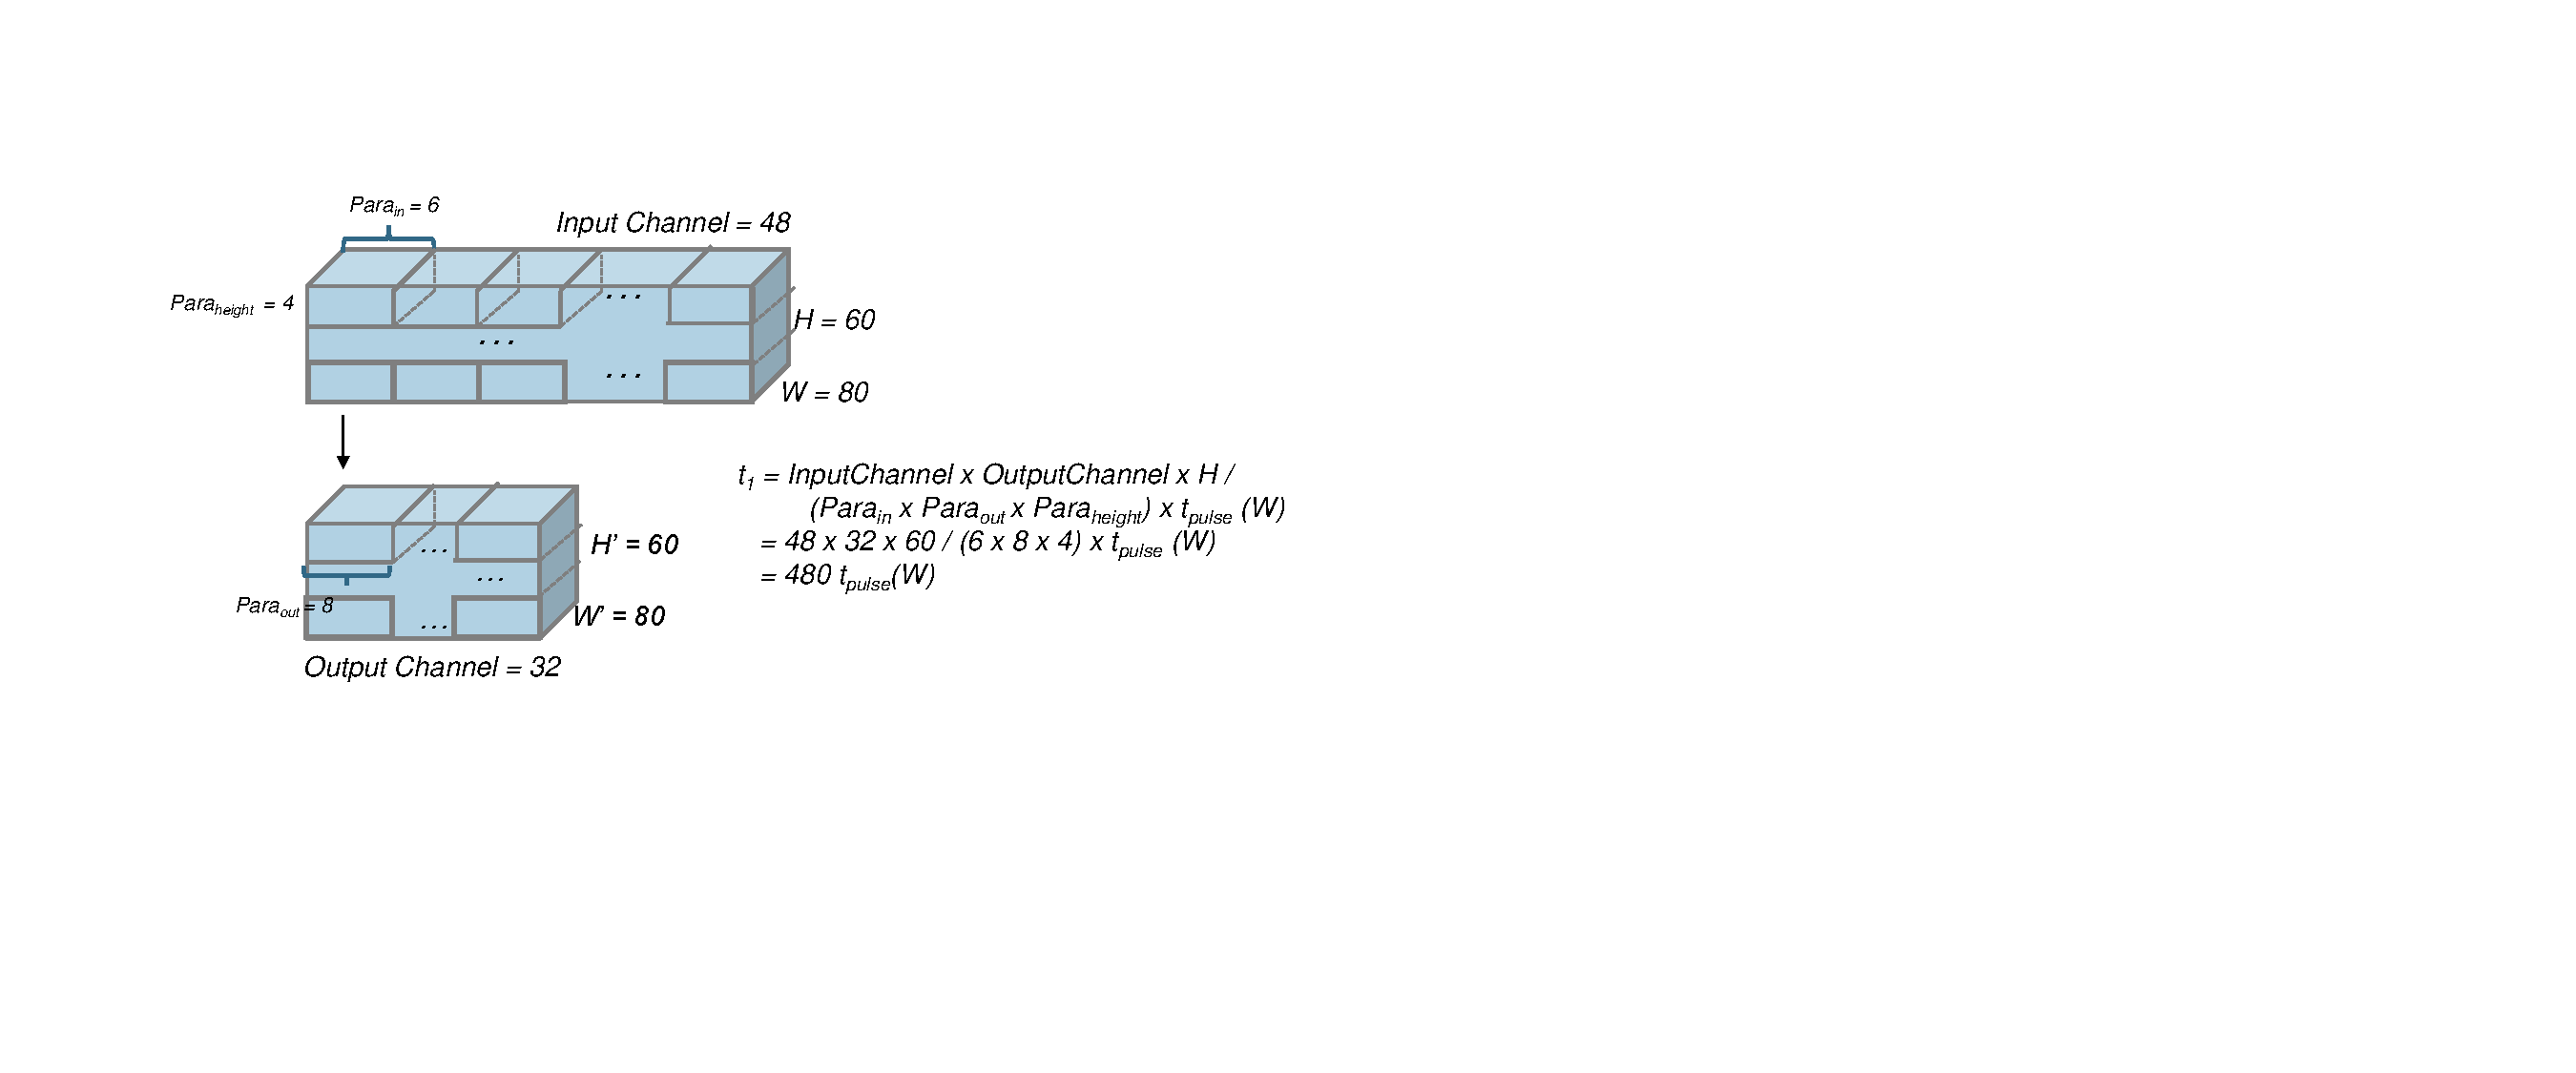
\includegraphics[width=0.99\linewidth]{fig/t1all.pdf}
% 		\end{minipage}%
% 	}
% 	\subfloat[ $t_1$ for Virtual-Instruction method. ]{ \label{fig:t1after}
% 		\begin{minipage}[t]{0.45\linewidth}
% 			\centering
% 	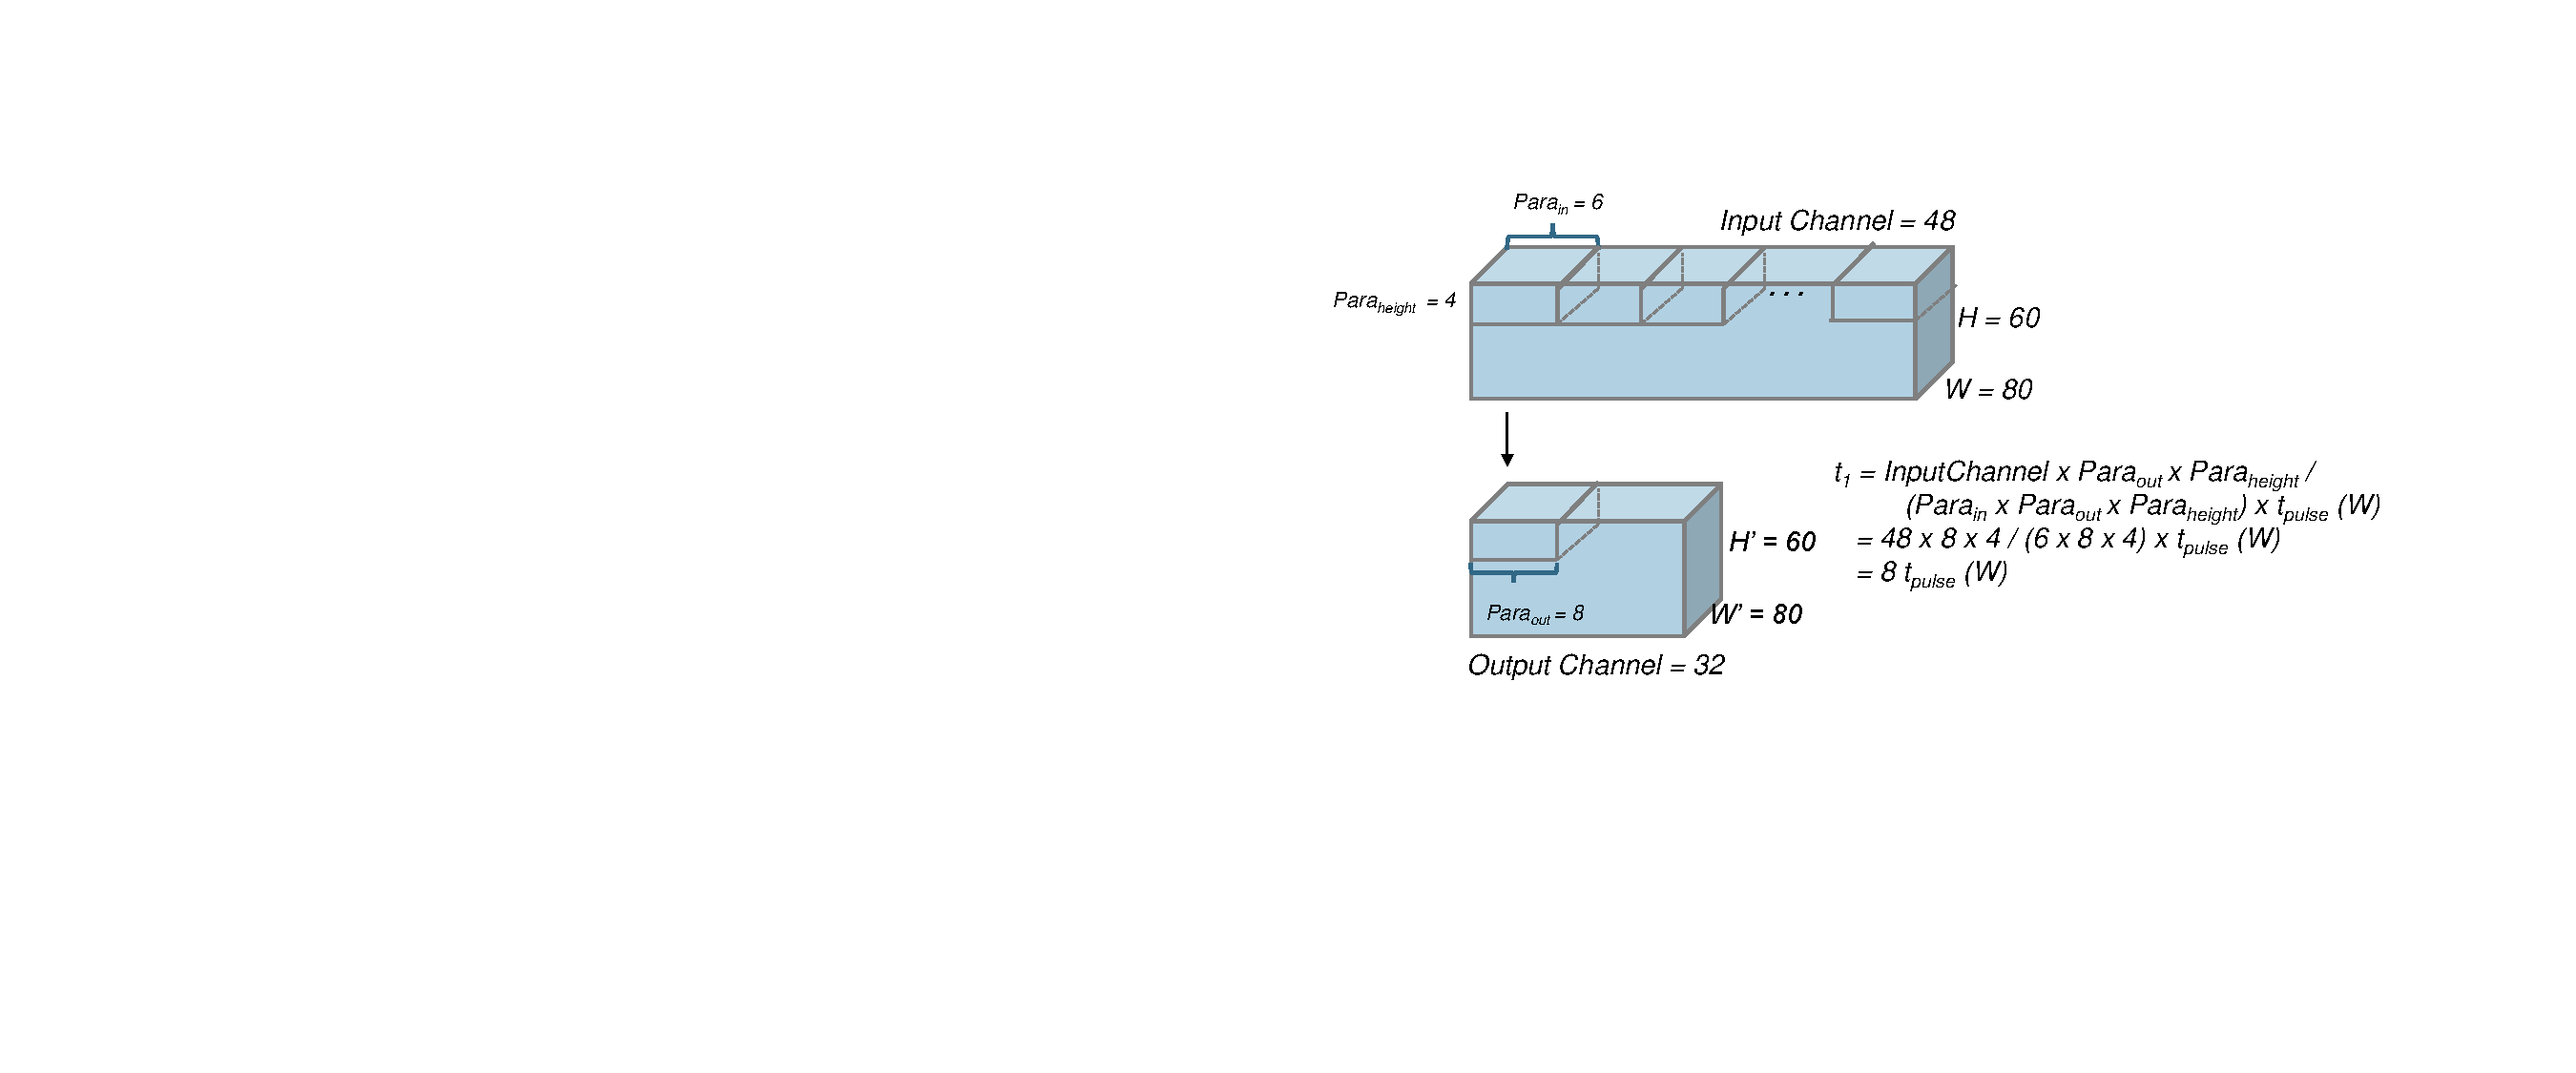
\includegraphics[width=0.99\linewidth]{fig/t1after.pdf}
% 		\end{minipage}%
% 	}
% 	\label{fig:t1example}
% 	\caption{ Waiting time for finishing the current operation ($t_1$) in an example convolution layer. Compared with the Layer-By-Layer method, the waiting time of our Virtual-Instruction method is reduced to $1.6\%$ in this example. The reduction in latency is related to the height ($H$) of the input featuremaps.  }
% \end{figure*}

Compared with Layer-by-layer interrupt, our method, which is interruptible after CALC\_F and SAVE, significantly reduces $t_{latency}$.
In the worst case, the interrupt request occurs at the beginning of the layer. In this case, the accelerator will wait until finishing the whole layer. The wait time is $t_{1\_layer}$:

\begin{equation*}
	t_{1\_layer} = \frac{ Ch_{in} \times Ch_{out} \times H }{ (Para_{in} \times Para_{out} \times Para_{height}) } \times t_{instr}(W)
\end{equation*}

Where $t_{instr}(W)$ is calculation time of a single CALC. The $W$ of the input featuremaps is larger, the time of a single CALC is longer.

The worst wait of our VI method is $t_{1\_VI}$:

\begin{equation*}
	t_{1\_VI} = \frac{ Ch_{in} \times Para_{out} \times Para_{height} }{ (Para_{in} \times Para_{out} \times Para_{height}) }  \times t_{instr}(W)
\end{equation*}

Compared with the Layer-By-Layer method, the worst latency of our method is reduced to $R_l$.

\begin{equation}
	R_l = \frac{ t_{1\_VI} }{ t_{1\_layer} }  = \frac{ Para_{out} \times Para_{height} }{ Ch_{out} \times H} 
	\label{equ:rate}
\end{equation}

The effect of latency reduction of the VI method is related to the number of output channels ($Ch_{out}$) and featuremap height ($H$). The larger the featuremaps output channels and the height, the better latency reduction result can be achieved.

For a medium-sized neural network layer, the input featuremap size is $80 \times 60$, the number of input channels is $CH_{in} = 48$, and the number of output channels is $CH_{out} = 32$. The instruction parallelism is restricted by the hardware architecture, whose input channel parallelism is $Para_{in} = 8$, output channel parallelism is $Para_{out} = 8$, height parallelism is $Para_{height} = 4$.
According to \Cref{equ:rate}, the latency is reduced to $\frac{ Para_{out} \times Para_{height} }{ Ch_{out} \times H} = 8 \times 4 / (32 \times 60) = 1.7\%$.

% An example of a convolution layer with a typical size in CNN is given in \Cref{fig:t1example}. The parameters are labeled in the figures. The latency can be reduced to $1.6\%$.

\subsection{ Instruction Arrangement Unit (IAU) }

Instruction Arrangement Unit (IAU) is the hardware to handle the computing requirements from tasks with different priorities. The IAU monitors the interrupt status and generates the original ISA instruction sequence. The original CNN accelerator does not need to know the interrupt status, and only operates the instructions provided by IAU.

The hardware implementation of IAU is shown in \Cref{fig:IAU}, which supports four tasks with different priorities. Task 0 has the highest priority and is not interruptible. 
InstrAddr records the address to fetch the instructions of the corresponding task. The InputOffset and the OutputOffset, which indicate base address offsets of the input and output data, are configured by the software. 
SaveID, SaveAddr, and SaveLength record the status when an interrupt occurs. 
Subsequent not-virtual SAVE instructions will be modified according to the recorded interrupt status (SaveID, SaveAddr, and SaveLength), to avoid duplicate output data transfer.



\begin{figure}[t]
	\centering
    % \vspace{-0.1cm} 
    % \setlength{\abovecaptionskip}{0cm} 
    % \setlength{\belowcaptionskip}{-0.4cm} 
	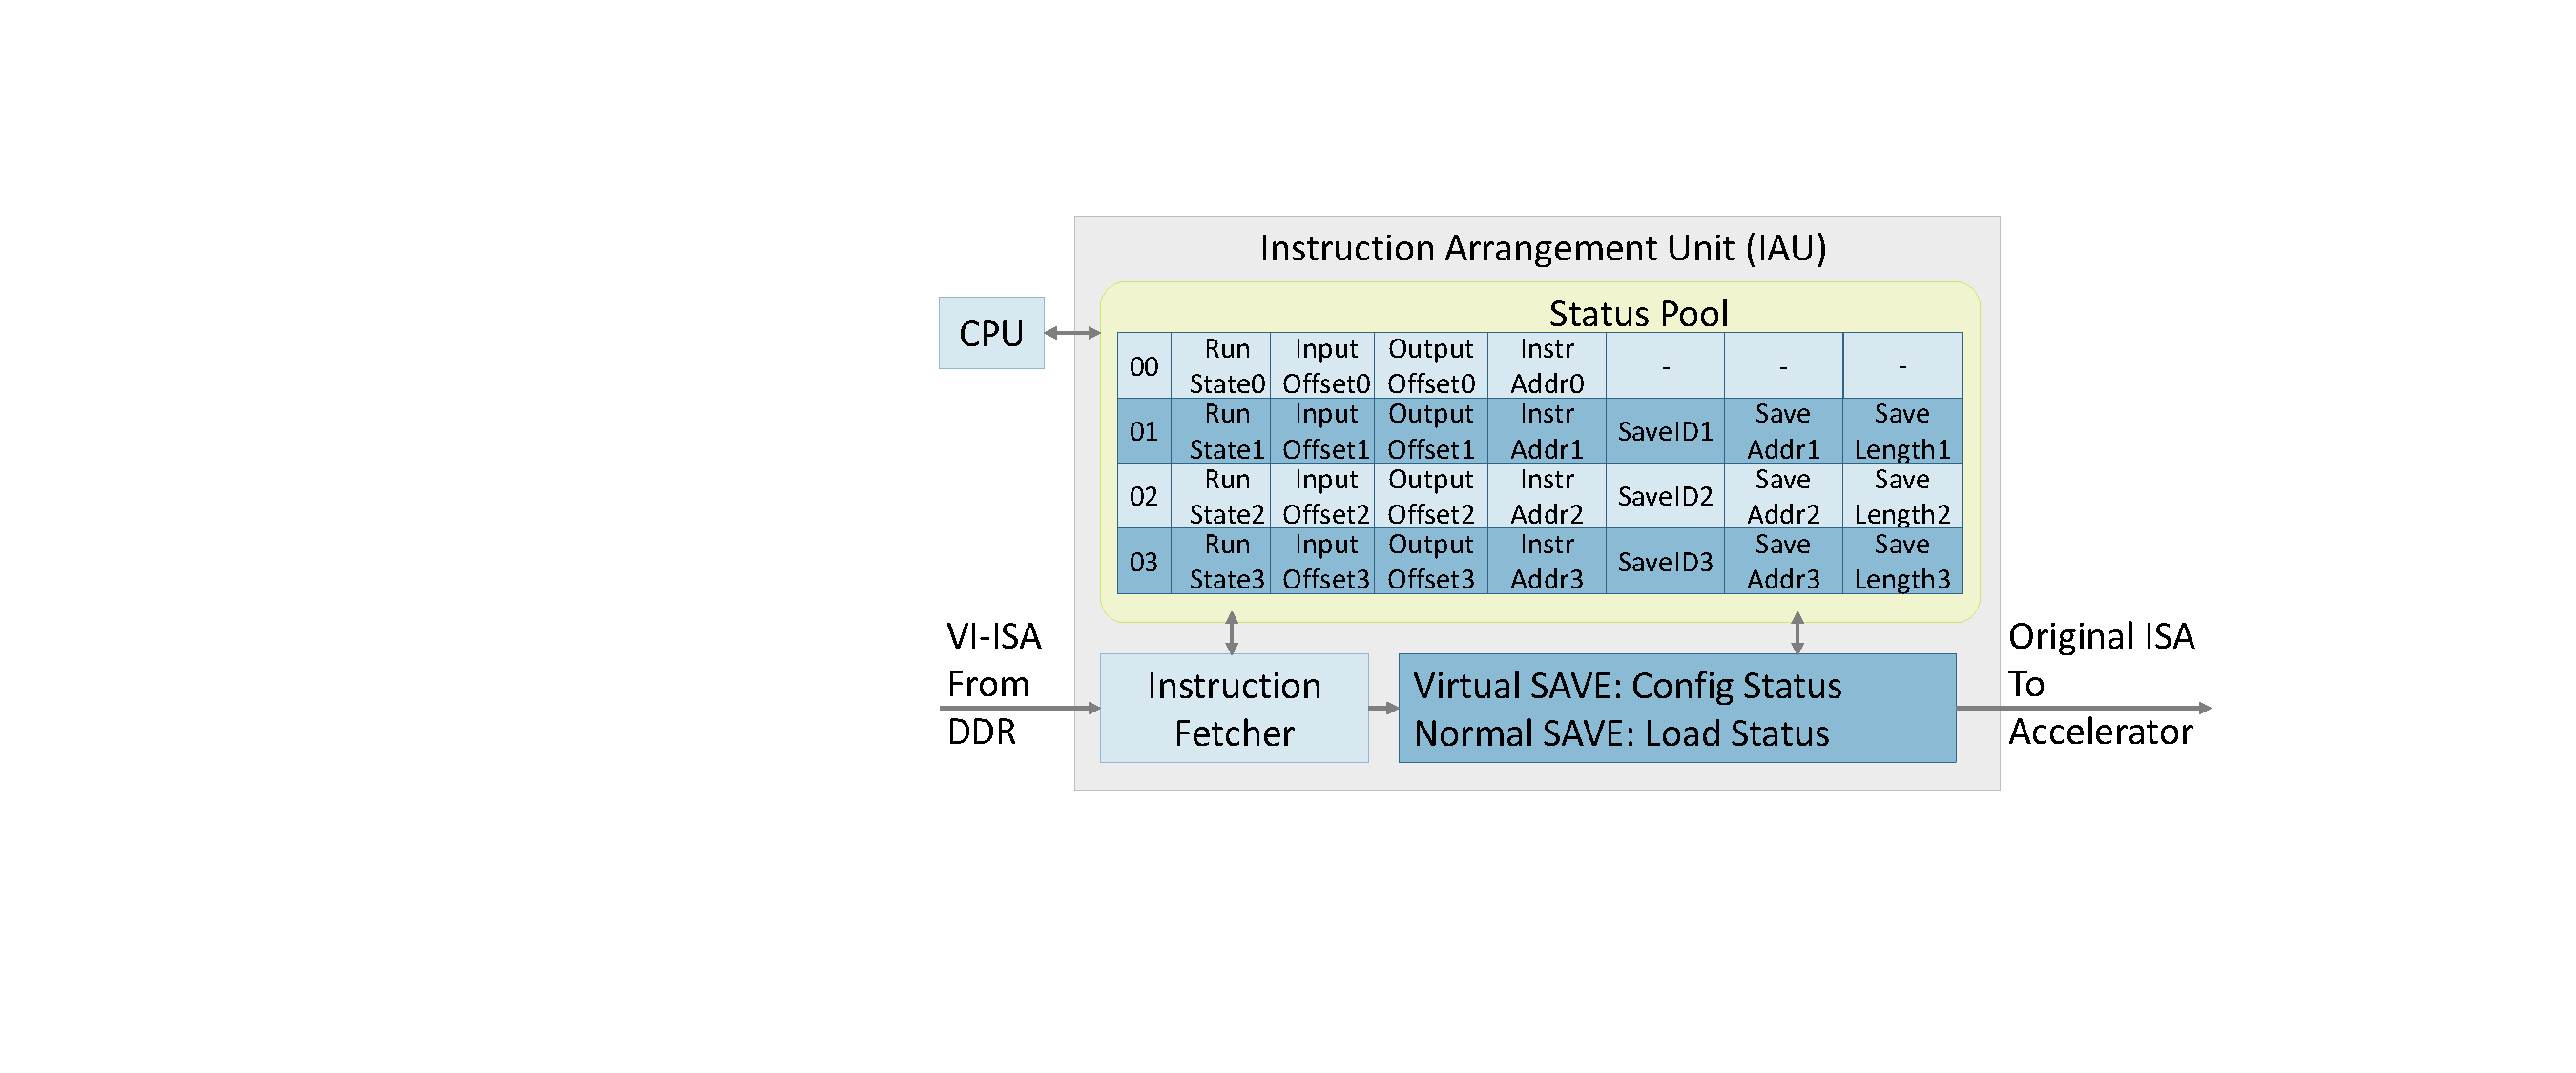
\includegraphics[width=0.9\linewidth]{fig/iau.pdf}
	\caption{Hardware architecture of IAU. 
	% The software on the CPU (PS side) communicates with IAU to access the CNN accelerator. IAU records the running state of each task. At runtime, IAU translates the input instruction sequence with virtual instructions to a normal sequence of instructions. IAU also modifies the normal SAVE instruction after interrupt occurs with the same SaveID, to avoid duplicate output data transfer. 
	}
	\label{fig:IAU}
\end{figure}

\begin{figure}[t]
	\centering
    % \vspace{-0.1cm} 
    % \setlength{\abovecaptionskip}{0cm} 
    % \setlength{\belowcaptionskip}{-0.05cm} 
	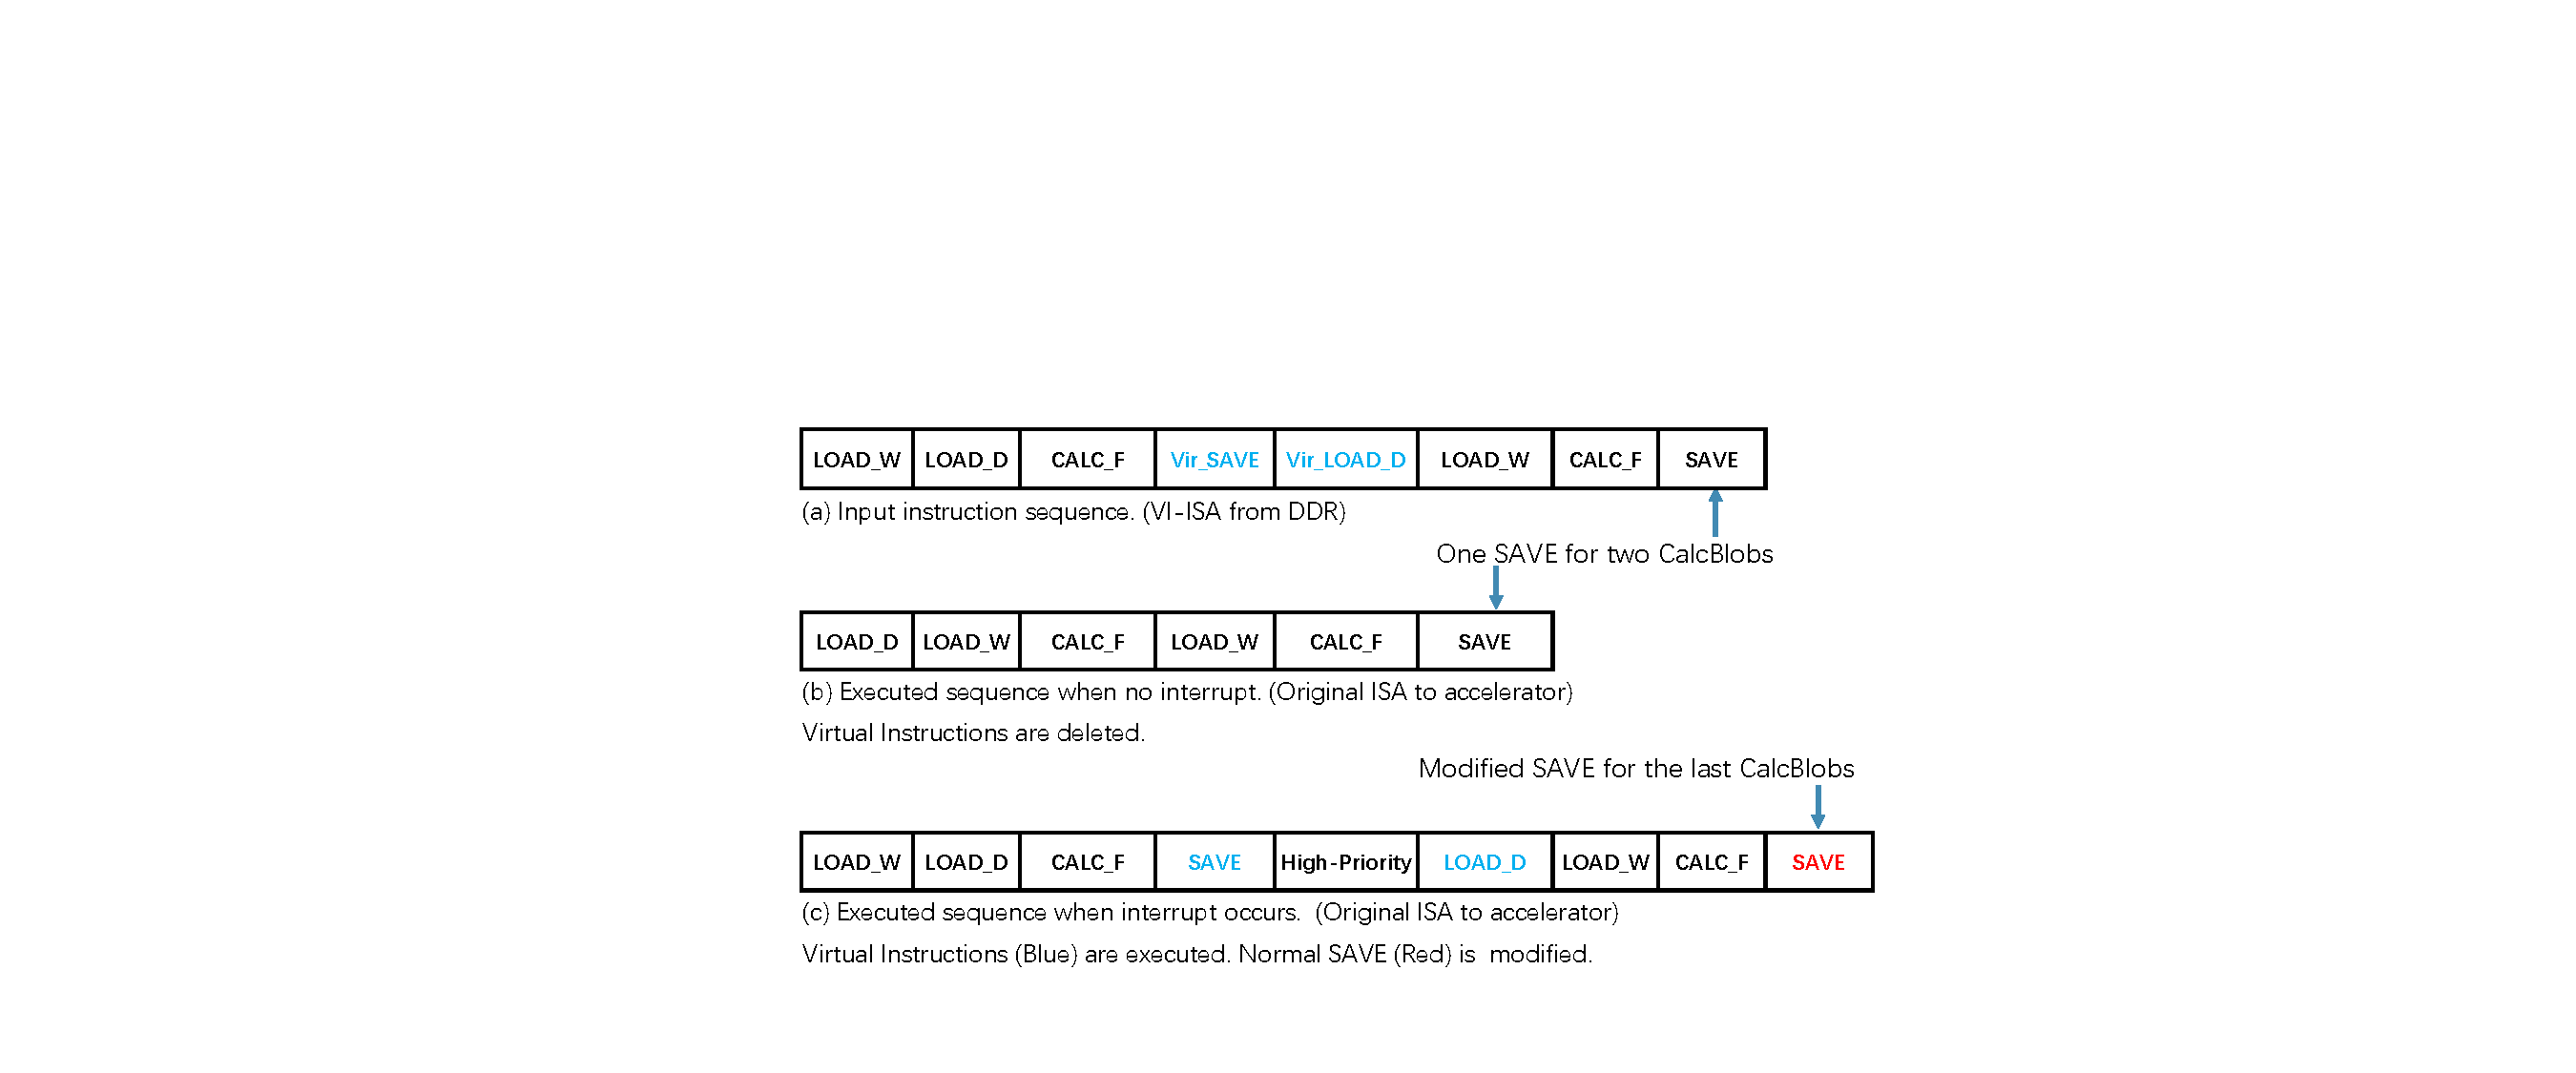
\includegraphics[width=0.9\linewidth]{fig/interexample.pdf}
	\caption{ A simple example of our proposed virtual-instruction-based interrupt. }
	\label{fig:interexample}
\end{figure}

\Cref{fig:interexample}(a) is the instruction sequence from DDR with VI-ISA. The instructions are generated for the scheduling shown in {fig:singlesave}. The Vir\_SAVE instruction is responsible for backing up executing status, i.e., saving the output results of the first CALC\_F. The Vir\_LOAD\_D instruction restore the input featuremaps from DDR to on-chip memory. The Vir\_LOAD. The SAVE instruction in \Cref{fig:interexample}(a) saves all the output results for the two CALC\_F.
\Cref{fig:interexample}(b) is the original ISA instructions translated by the IAU without interrupt. The virtual instructions (Vir\_SAVE and Vir\_LOAD) are skipped and discarded by the IAU. Thus the accelerator receives the original ISA sequence without backup or restore instructions.
When an interrupt occurs at the first CalcBlob, \Cref{fig:interexample}(c) illustrates the backup/recovery instructions (Blue) and the modified SAVE instruction (Red). Because the output results of the first CALC\_F are stored to DDR with the fitst SAVE, which is translated from the Vir\_SAVE in fig(a), the last SAVE instruction is modified to only store the output results of the second CALC\_F.

\section{Evaluation and Results}
\label{sec:experiments}




% In this section, the evaluation of the instruction-based-interruption, hardware modules for FE post-processing, and the overall DSLAM system are presented and analyzed.



\subsection{ Experiment Setup }

The hardware-in-loop evaluate environment is illustrated in \Cref{fig:env}(a). There is a simulation server providing the simulation environment based on AirSim \cite{shah2018airsim}. The AirSim simulator provides the camera data for the two agents. Two Xilinx ZCU102 boards \cite{zcu102}, with ZU9 MPSoC \cite{MPSoC}, are responsible for the calculation of each agent.
SuperPoint \cite{detone2018superpoint} is used for extracting feature-points. GeM \cite{radenovic2018fine} is used to implement the PR module.

The CNN is calculated by the Angel-Eye CNN accelerator \cite{guo2017angel} on the FPGA side of ZU9 MPSoC, and other operations are on the CPU side.
For a precise evaluation of the CNN running time, we record the clock cycles of the beginning and end of each instruction. The time of the interrupt response latency and the total cost in the following evaluation is calculated from the clock cycles and the clock frequency. The CNN accelerator and the IAU are running at 300MHz.

% The hardware resources are listed in \Cref{tab:hardware}. The hardware resources are provided by Vivado after hardware implementation. Vivado \cite{Vivado} is the development toolchain for MPSoC provided by Xilinx. The CNN backbone is calculated by the Angel-Eye CNN accelerator \cite{guo2017angel} on the FPGA side of ZCU102 (Programmable logic, PL side). The FE post-processing steps run on our proposed accelerators, also on the PL side. The PL side has 2 clock frequencies. The CNN accelerator and the IAU are running at 300MHz. The accelerator for FE post-processing is running at 200MHz. Compared with the CNN accelerator, IAU and FE post-processing use very little hardware resources.

% % Table generated by Excel2LaTeX from sheet 'Sheet1'
% \begin{table}[t]
% \centering
% % \setlength{\abovecaptionskip}{2pt}
% \caption{Hardware consumption of the proposed hardware}
% % Table generated by Excel2LaTeX from sheet 'Sheet1'
% \begin{tabular}{|c|c|c|c|c|}
% \hline
% & $\# DSP$ & $\# LUT$ & $\# FF$ & $\# BRAM$ \\
% \hline
% On-Board resource & 2520 & 274080 & 548160 & 912 \\
% \hline
% CNN accelerator & 1282 & 74569 & 171416 & 499 \\
% \hline
% IAU & 0 & 2268 & 4633 & 4 \\
% \hline
% FE post-processing & 25 & 17573 & 29115 & 10 \\
% \hline
% \end{tabular}%
 
% \label{tab:hardware}%
% \end{table}%

% \begin{figure}[t]
% \centering
% % \vspace{-0.1cm} 
% % \setlength{\abovecaptionskip}{0cm} 
% % \setlength{\belowcaptionskip}{-0.05cm} 
% 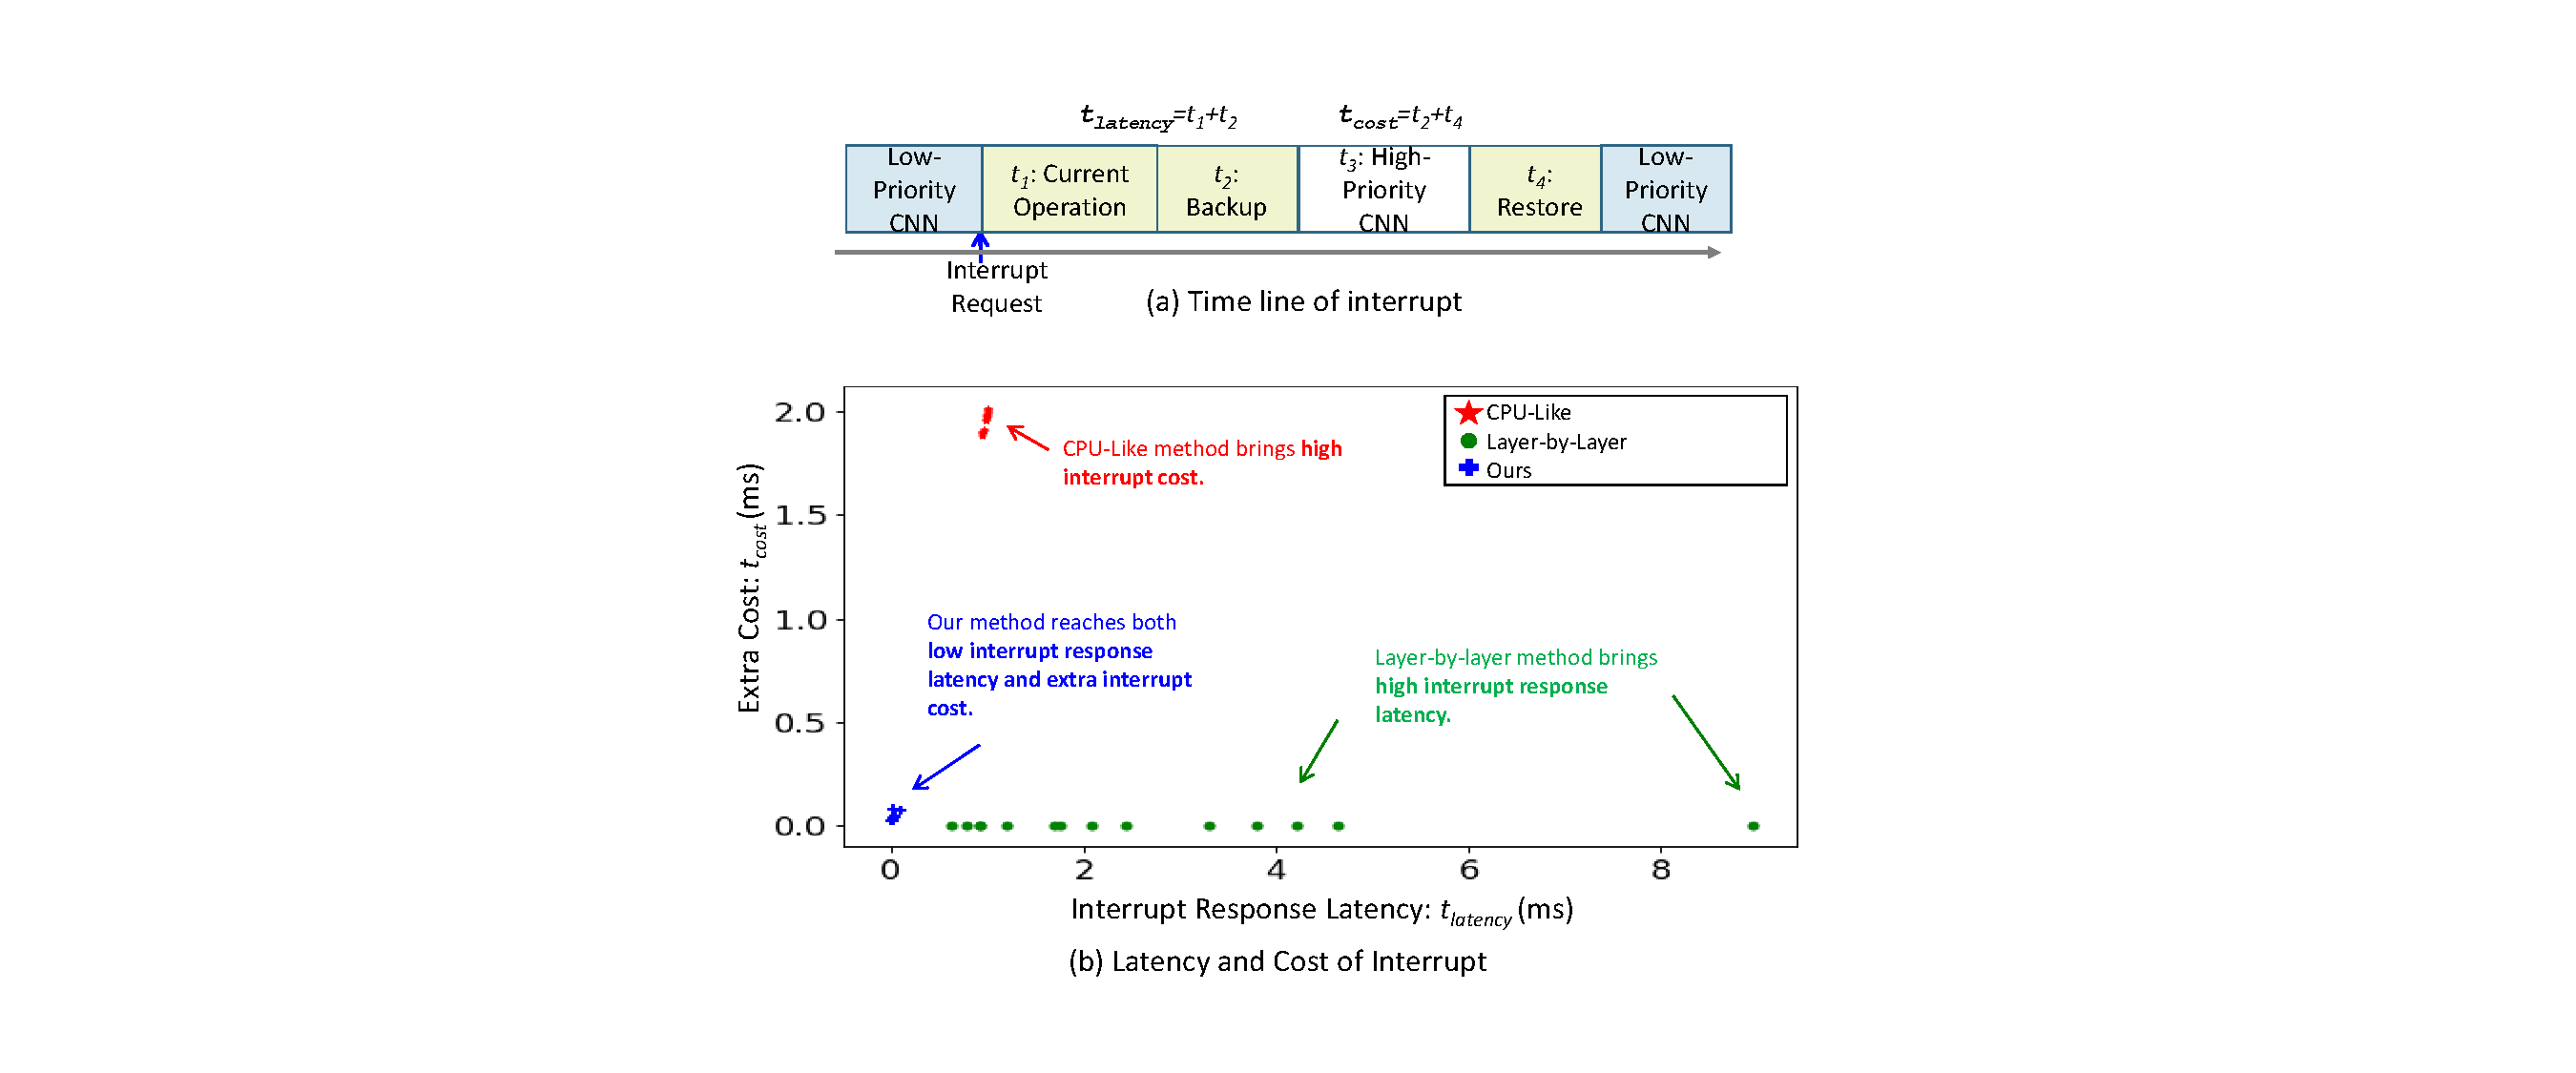
\includegraphics[width=0.99\linewidth]{fig/PRresult.pdf}
% \caption{The interrupt response latency \& extra time cost.}
% \label{fig:scatter1024}
% \end{figure}


\subsection{Virtual Instruction-based interrupt }

In DSLAM, only the low-priority PR task is interruptible, and the interrupt position is unpredictable. GeM \cite{radenovic2018fine} is used to implement the PR module in the experiment.
The CNN backbone of the GeM is ResNet101 \cite{he2016deep}, which contains 101 convolution layers. The input shape of the CNN is $480 \times 640 \times 3$. The parallelism of the Angel-Eye is $Para_{height}=8$, $Para_{in}=16$, $Para_{out}=16$. 
We randomly sample 12 positions of the ResNet101 CNN backbone. The interrupt response latency and the extra time cost for different implementation of interrupt at the positions are listed in \Cref{fig:barresult}(a).
The CPU-like interrupt consumes the most extra cost ($t_{cost}$). Though the layer-by-layer interrupt consumes no extra time, the latency is much higher than our virtual-instruction-based interrupt. 
This is because the layer-by-layer interrupt needs to wait for the completion of a layer. The performance at the same interrupt position in our proposed virtual interrupt can interrupt inside a layer, with lower latency.

\label{sec:viexp}

Furthermore, though the network structures differ between different CNNs, the convolutional layers, which are the basic component in CNN, are similar between different CNNs. INCA monitors the running status inside each layer, and the interrupt respond latency and extra cost are only relevant to the currently operating layer. 
We compare the interrupt respond latency of our VI method with layer-by-layer method at different layers from different networks, including ResNet \cite{he2016deep}, VGG \cite{simonyan2014very}, and MobileNet \cite{howard2017mobilenets}. The results is illustrated in \Cref{fig:barresult}(b). We evaluate our method on both th big accelerator with large hardware parallelism and small accelerator with small parallelism. 
In the ResNet and VGG, the average interrupt respond latency of the layer-by-layer method is $ms$ to tens of $ms$, which makes the high priority task with hard deadline in the embedded system unable to be completed on time. With our VI method, the latency can be reduced to less than 100$us$, so that the high priority task can be started immediately and completed on time. 
For the lightweight network (MobileNet), although the latency of the layer-by-layer method is about 1ms, we can still reduce the latency by 2-3 orders of magnitude with VI method. This result also matches the theoretical analysis in \Cref{equ:rate}.



% The latency to respond the interrupt in CPU-like method consists of the time to finish current executing instruction and the data backup time ($t_{latency} = t_1+t_2$) for the on-chip data/weights caches (totally 2.2MB). The latency in layer-by-layer interrupt is the time to finish current layer. The latency of our virtual-instruction-based method is the time to finish current executing instruction and the backup time for the calculated output results. 
% The cost of CPU-like interrupt is the data transfer time of all the on-chip caches (totally 2.2MB) to/from DDR ($t_{cost} = t_2+t_4$). The cost of virtual-instruction-based method is only the recovery of the input/weights from DDR to on-chip caches ($t_{cost} = t_4$). There is no extra cost for the layer-by-layer interrupt.

% 


% \subsubsection{ Time comparison between $t_1$ and $t_2$ }

% As described in \Cref{sec:virtualinstr}, the layer-by-layer interrupt method do not need to backup data before interruption ($t_2 = 0$). Though our Virtual-Instruction method (VI method) need to spend time to backup the final results, which are already generated yet not stored to DDR ($t_2$). However, compared with computation, the time of data backup ($t_2$) is short. We list the backup time and the convolution time ($t_1$) at some of the interrupt position in \Cref{fig:scatter1024}(b), with different featuremap shape, kernel size, and input/output channels. $H$, $W$ are the height, width of input featuremaps. $Ch_{in}$, $Ch_{out}$ are the number of input and output channels. The time of backup and calculation is listed in $Backup$ and $Conv$ columns. The ratio of backup and calculation are listed in the last column. The backup operation only consumes less than 20\% of the calculation time. For the first layer (first line of \Cref{tab:timecompare}). The input channels number is too small, so the calculation time is also short. Therefore, the backup time has reached half of the calculation time. 

% % Table generated by Excel2LaTeX from sheet 'Sheet4'
% \begin{table}[t]
% \centering
% % \footnotesize
% \caption{Time comparison between data backup and calculation}
% \begin{tabular}{|c|c|c|c|c|c|c|c|}
% \hline
% \multirow{2}[2]{*}{$H$} & \multirow{2}[2]{*}{$W$} & \multirow{2}[2]{*}{$Ch_{in}$} & \multirow{2}[2]{*}{$Ch_{out}$} & Kernel & Backup & Conv & \multirow{2}[2]{*}{$\frac{Backup}{Conv}$} \bigstrut[t]\\
% & & & & Size & ($t_2$,$us$) & ($t1$,$us$) & \\
% \hline
% 480 & 640 & 3 & 64 & $7 \times 7$ & 26.29 & 52.38 & 50.2\% \\
% \hline
% 120 & 160 & 128 & 128 & $3 \times 3$ & 8.77 & 41.18 & 21.3\% \\
% \hline
% 30 & 40 & 1024 & 2048 & $1 \times 1$ & 1.25 & 8.75 & 14.3\% \\
% \hline
% 30 & 40 & 512 & 512 & $3 \times 3$ & 1.42 & 39.36 & 3.6\% \\
% \hline
% 16 & 20 & 512 & 512 & $3 \times 3$ & 0.75 & 20.16 & 3.8\% \\
% \hline
% \end{tabular}%
% \label{tab:timecompare}%
% \end{table}%


\subsection{ ROS based DSLAM }


The results of the DSLAM based on INCA is shown in \Cref{fig:env}. The space in the AirSim \cite{shah2018airsim} for the robots to explore is shown in \Cref{fig:env}(a). It is a simple rectangle area with four different pillars, and some chairs at the center (in the white box). \Cref{fig:env}(b) shows how PR works for map merging. The visual odometry (VO) based on feature-points on each agent produces the local map and trajectory. When the PR threads find out a similar scene, and the maps and the trajectories are merged via the similar scene, as shown in \Cref{fig:env}(c).

In this example, the CNN-based feature-point extraction (FE) and place recognition (PR) are both executed on the same Angel-Eye \cite{guo2017angel} accelerator. The frequency of the input camera is 20fps, and each input frame is fed to the FE, and the FE module would take up the accelerator. While the CPU process VO with the feature-points from FE, the accelerator can switch to process the low-priority PR task, as illustrated in \Cref{fig:inca}(a). Thus, the PR process one frame every 7$\sim$10 input frames.
However, the scene between adjacent frames is similar, so it is not necessary to do place recognition for each input picture. Place recognition every 10 frames can meet the task requirements of DSLAM.

\section{Conclusion}
\label{sec:conclusion}

In this paper, we propose an interruptible CNN accelerator and a deployment framework, INCA. 
With the help of the virtual-instruction-based interrupt method (VI method), the CNN accelerator can switch between different CNN tasks with low interrupt response latency and low extra cost. 
INCA only needs to modify the instruction fetch module to IAU in hardware. Thus, it is easy to extend to different instruction-driven accelerators.
% Note that the development of CPU task scheduling evolved from single-core multi-tasking to multi-core multi-tasking. 
% Similarly, 
INCA currently focuses on interrupt support for single-core multi-tasking. 
We plan to investigate the multi-core multi-tasking for CNN accelerators as part of future work.
% Therefore, with the help of INCA, the independent software in ROS can access the accelerator without hardware resources conflicts, on various CNN accelerators.

\bibliographystyle{IEEEtran}
\bibliography{src/fpgaslam}


% \begin{thebibliography}{00}
% \bibitem{b1} G. Eason, B. Noble, and I. N. Sneddon, ``On certain integrals of Lipschitz-Hankel type involving products of Bessel functions,'' Phil. Trans. Roy. Soc. London, vol. A247, pp. 529--551, April 1955.
% \bibitem{b2} J. Clerk Maxwell, A Treatise on Electricity and Magnetism, 3rd ed., vol. 2. Oxford: Clarendon, 1892, pp.68--73.
% \bibitem{b3} I. S. Jacobs and C. P. Bean, ``Fine particles, thin films and exchange anisotropy,'' in Magnetism, vol. III, G. T. Rado and H. Suhl, Eds. New York: Academic, 1963, pp. 271--350.
% \bibitem{b4} K. Elissa, ``Title of paper if known,'' unpublished.
% \bibitem{b5} R. Nicole, ``Title of paper with only first word capitalized,'' J. Name Stand. Abbrev., in press.
% \bibitem{b6} Y. Yorozu, M. Hirano, K. Oka, and Y. Tagawa, ``Electron spectroscopy studies on magneto-optical media and plastic substrate interface,'' IEEE Transl. J. Magn. Japan, vol. 2, pp. 740--741, August 1987 [Digests 9th Annual Conf. Magnetics Japan, p. 301, 1982].
% \bibitem{b7} M. Young, The Technical Writer's Handbook. Mill Valley, CA: University Science, 1989.
% \end{thebibliography}
% \vspace{12pt}
% \color{red}
% IEEE conference templates contain guidance text for composing and formatting conference papers. Please ensure that all template text is removed from your conference paper prior to submission to the conference. Failure to remove the template text from your paper may result in your paper not being published.

\end{document}
